\chapter{Implementation}

%The implementation should look at any issues you encountered as you tried to implement your design. During the work, you might have found that elements of your design were unnecessary or overly complex, perhaps third party libraries were available that simplified some of the functions that you intended to implement. If things were easier in some areas, then how did you adapt your project to take account of your findings?

%It is more likely that things were more complex than you first thought. In particular, were there any problems or difficulties that you found during implementation that you had to address? Did such problems simply delay you or were they more significant? Your implementation might well be described in the same chapter as Problems (see below).

\section{Prototype}
Building a prototype will quickly highlight the main flaws in the initial design.  This is not the same as the intended final version and in this case is not even the same materials as I have chosen.  It does however confirm the basic design but is made from much cheaper sourced components.  I already had an Arduino Uno (the basic prototyping model) from my interest in the technology before I attended university, so this was an easy component to acquire quickly and is perfect for a prototype.  I had no chassis built or any materials to make one so I found a cheap and easy to assemble one online at a hobbyist electronics retailer.  This kit also included some very small DC motors with gearboxes and wheels, very convenient little package.  The Arduino along with the chassis kit and a small infrared sensors, a 9 volt battery and some jumper wires and a prototype was put together in a short period of time.
\begin{figure}[H]
\centering
        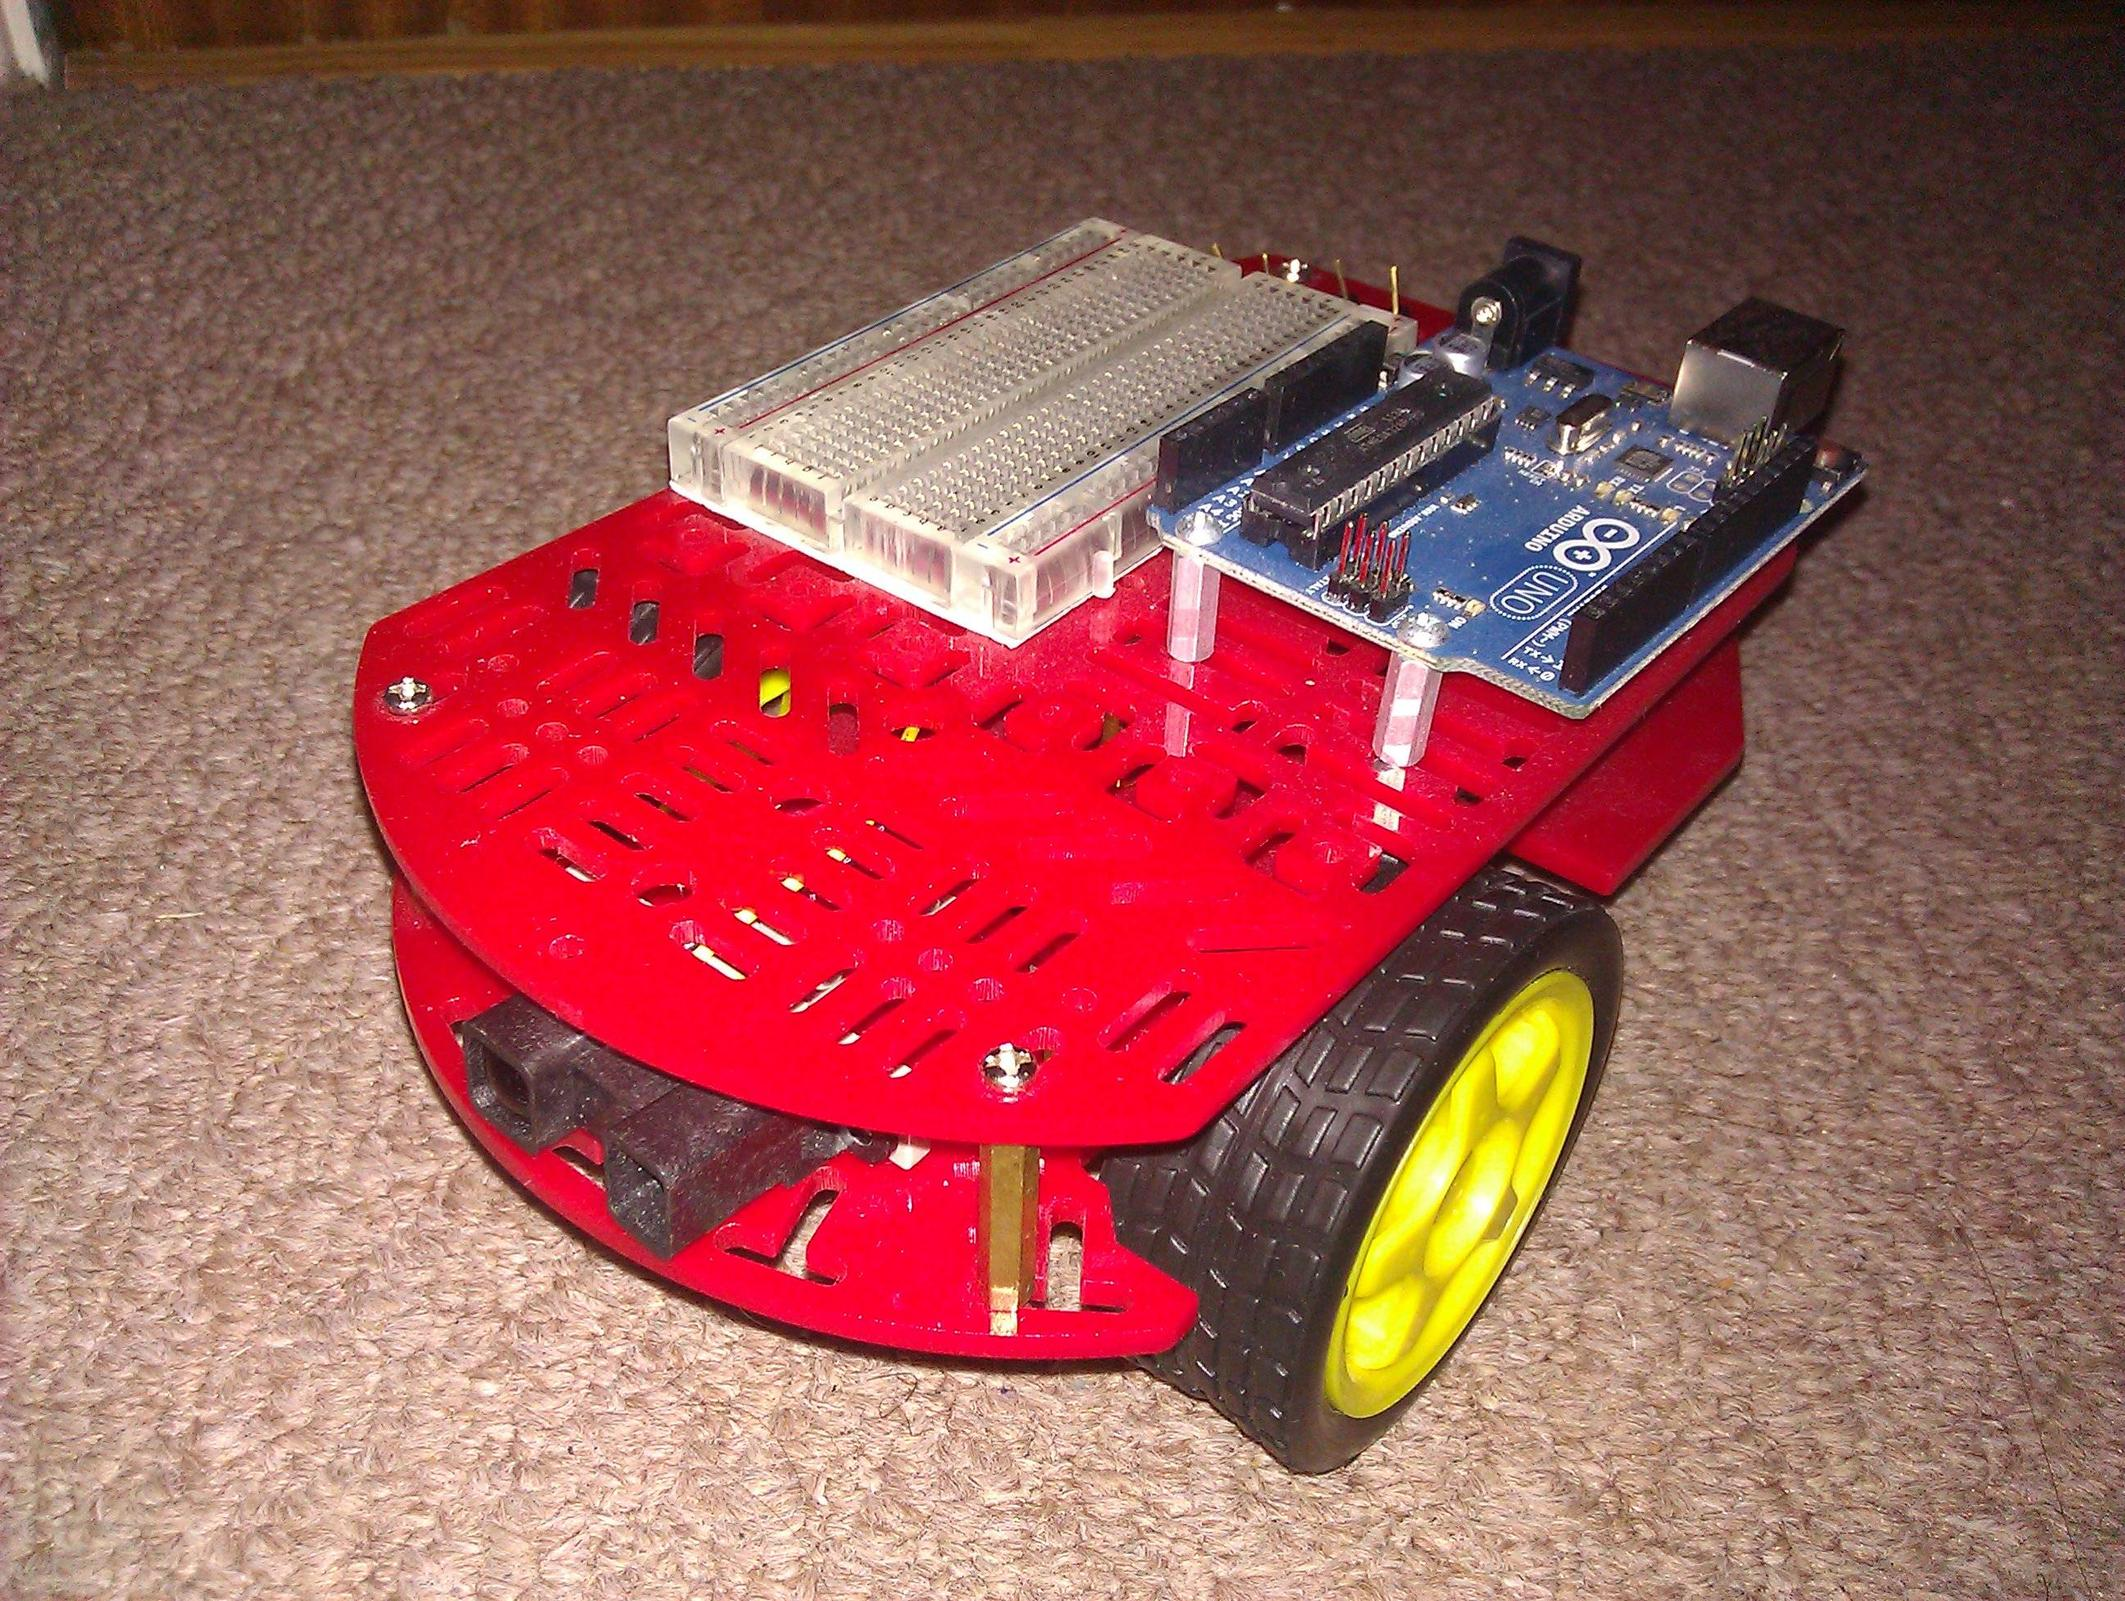
\includegraphics[width=3.0in] {Images/tria-mkI.jpg}
        \caption{Prototype mkI}
        \label{Prototype mkI}
\end{figure}

Wiring up the components was fairly easy due to there only being two motors and a single infrared sensor.  The sensor just has 3 pins, ground and positive power pins as well as a signal pin.  This is basically set up like a resistor, you supply power to the positive pin, attach the ground to the ground power rail of the system and just read the value being transmitted back on the signal pin.  The difference between zero up to the amount of power being given to the sensor, in this case the data sheet specified 5 volts as the upper edge and that is what I supplied the sensor with, gives an indication of how far it is from an object.  With this sensor the higher value returned is actually how close the object is and the lower number indicates it is further away.  This is due to the fact that the reading received is indicating how intense the amount of infrared getting back to the sensor is.
\\The harder part of this was getting the motors to run safely, this issue was discovered when putting together this prototype and testing each part as it was implemented.  The Arduino I use for prototyping can only output a regulated voltage of 3.3 or 5 volts.  The motors supplied with the chassis kit do not run very well at this voltage and struggle to move on thick carpet.  As the supply I am using to power the Arduino is a 9 volt battery this was sufficient to run the motors at an acceptable level, the only problem is supplying this to both the Arduino and the motors.  As the microcontroller is needed to control when and how fast the motors are to turn, simply wiring the power supply directly to the motors is a bad idea as they will just spin constantly due to always having power.
\begin{figure}[H]
\centering
        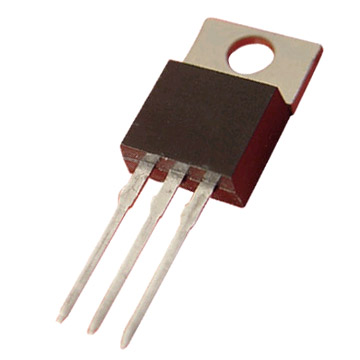
\includegraphics[width=2.0in] {Images/transistor.jpg}
        \caption{Transistor - zmescience.com}
        \label{Transistor}
\end{figure}

This could be solved using a transistor (a semiconductor device used to switch electrical signals) by supplying it with the higher voltage, connecting it to the motor and when a signal voltage from the Arduino is received it switches to the higher voltage allowing the motor to turn.  This is a very handy little component which is at the core of modern day electronics, but to use it in this fashion would need a lot more complicated circuitry as to ensure that this higher voltage does not damage other components in the circuit.  Another solution would be to use a chip known as a h-bridge.
\\This chip also acts like a switch but with the addition that it can change the currents direction meaning that you can not only control when the motor is on or off but also the direction it turns without additional complex circuitry.
\begin{figure}[H]
\centering
	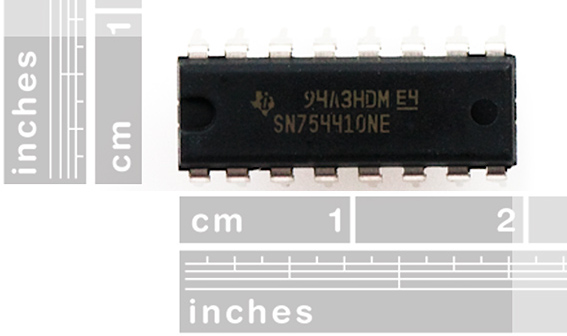
\includegraphics[width=2.0in]  {Images/h-bridge.jpg}
	\caption{H-Bridge - sparkfun.com}
	\label{H-Bridge}
\end{figure}
I discovered that the h-bridge chip also has its issues, as it generates heat when high currents are passed through it so if the motors are working hard more current will be drawn and the more heat the chip will generate and possibly burn out.  There is again the issue of having no protection for the rest of the circuit.  An option that would solve this issue is a full motor driver board but the cost if these is many times the cost of the components to make the circuits myself.  For example a h-bridge chip an assortment of diodes, capacitors, resistors and transistors costs around \pounds5 while a fully built board costs around \pounds20-30.
\begin{figure}[H]
\centering
        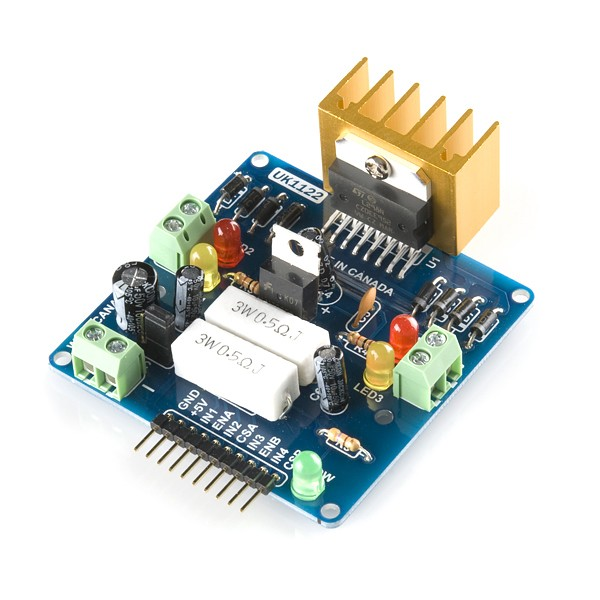
\includegraphics[width=2.0in]  {Images/motor-driver.jpg}
        \caption{Motor Driver - sparkfun.com}
        \label{Motor Driver}
\end{figure}
I decided to build a simple motor driver using the h-bridge chips, effective for a simple prototype.
\\With only a single infrared sensor the only logical place to mount it would be to have it facing directly forwards.  After writing the code to control the motors and process readings taken from the front mounted sensor the logic to test the concept is very simple.  Just check if there is something close in front and if there is just turn and check again, if there is not just keep moving forwards.
The logic looks like this:
\begin{figure}[H]
\begin{lstlisting}[basicstyle=\ttfamily]
if(sensor_range < value)
{
	motors.turn.right(45);
}else
{
	motors.move.forward(1);
}
\end{lstlisting}
\caption{Prototype Code Exert}
\label{Prototype Code Exert}
\end{figure}
This seems to work quite well, it does drive forwards and it does turn when an object comes in range of the infrared sensor.  This is the desired behaviour but there is a problem.  If the robot turns away from one object and into another, if that second object is too close by the time it comes in front of the sensor then it can not be seen by the sensor.  The sensor that I have fitted to the prototype has a maximum range of 150cm, but it also has a minimum range of 20cm meaning that is blind to any object closer than this minimum range.
\\In the figure the red signifies the blind area of the sensor and the green is the visible area.  If the robot were to turn right to avoid the wall in front of it then it would collide with the other wall and not be able to detect it.
\begin{figure}[H]
\centering
        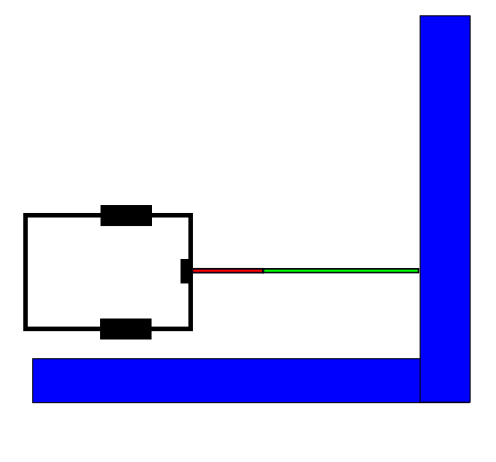
\includegraphics[width=3.0in]  {Images/ir-demo.png}
        \caption{Collision Illustration}
        \label{Collision Illustration}
\end{figure}
Another issue with the prototype robot is with the motors.  Even though I am supplying each motor with the same voltage they do not turn at the same speed, this is due to the lack of feedback with controlling them.  Also the fact that it is built from a very cheap kit is a probable reason for how uneven the speed of the motors is.  This all leads to the robot driving in a curve as opposed to the intended straight line, also contributing to the sensor problem of turning into an object putting it within the sensor blind spot.
\subsection{Prototype Evaluation}
The main issues with the prototype are the motors and the lack of more than a single sensor.
\\The motors did not run at exactly the same speed causing the robot to turn constantly as well as having no feedback system connected to the motors or the wheels and as such the robot nor the user know what position the drive system is in or how far the robot has moved.
\\Having just a single sensor facing directly forwards highlighted the need for more sensors covering a wider area in front of the robot due to when turning objects may be moved into the blind spot of the sensor and not be seen causing a collision.
\\These issues were taken into consideration when designing the second iteration of the robot.

\section{MK-I}
The next step was to build a version based on the design and using the things that were learnt from the prototype to improve it.
\\First thing to do was to build a sturdy chassis for all the systems to be mounted onto.  I bought several sheets of aluminium to but cut into a similar shape as the small red plastic prototype.
\begin{figure}[H]
\centering
        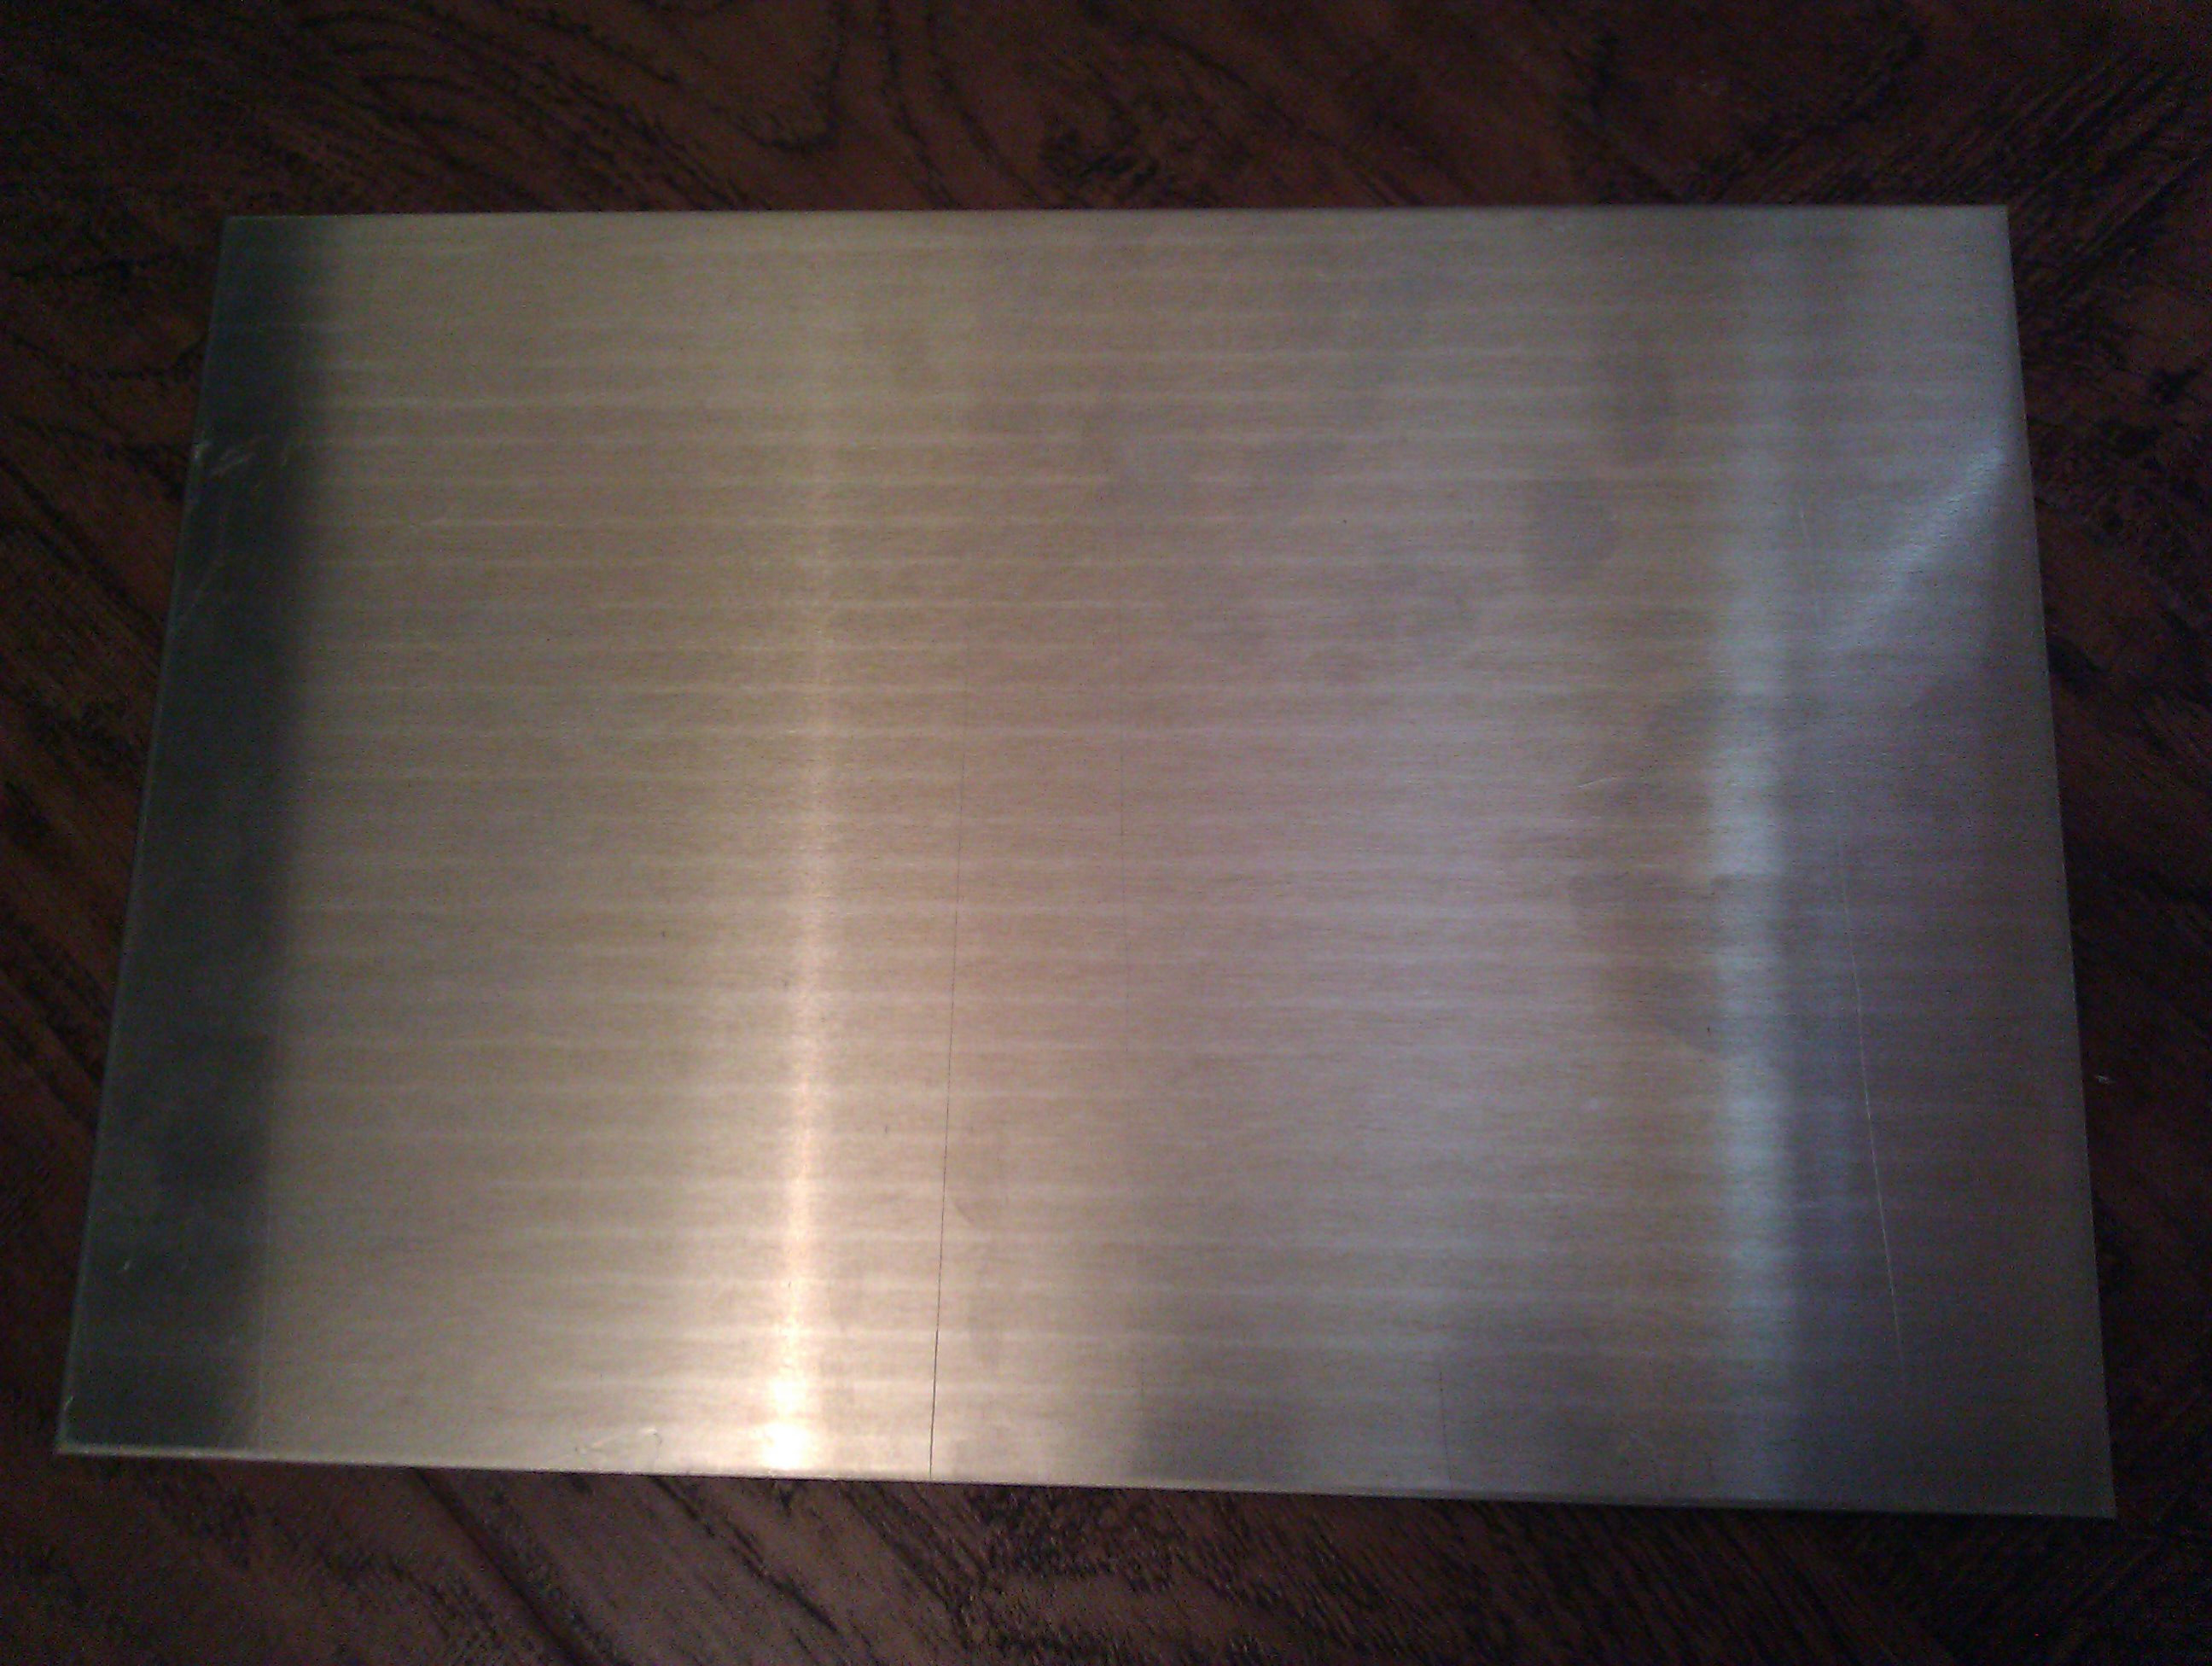
\includegraphics[width=3.0in]  {Images/alu-sheet-2.jpg}
        \caption{Aluminium Sheet}
        \label{Aluminium Sheet}
\end{figure}
I chose this shape mainly because of how much I liked working with the kit used in making the prototype.  Even though the first version was not perfect, the sensor was successful to a certain degree, it just needed more of them to cover the blind spots.  The curved shape of the front where the sensors mounted makes sense because then each sensor reading will provide the same relative distance from the robot unlike if it was square than the edge would be closer to the object in the environment than the robot thinks.
\begin{figure}[H]
\centering
        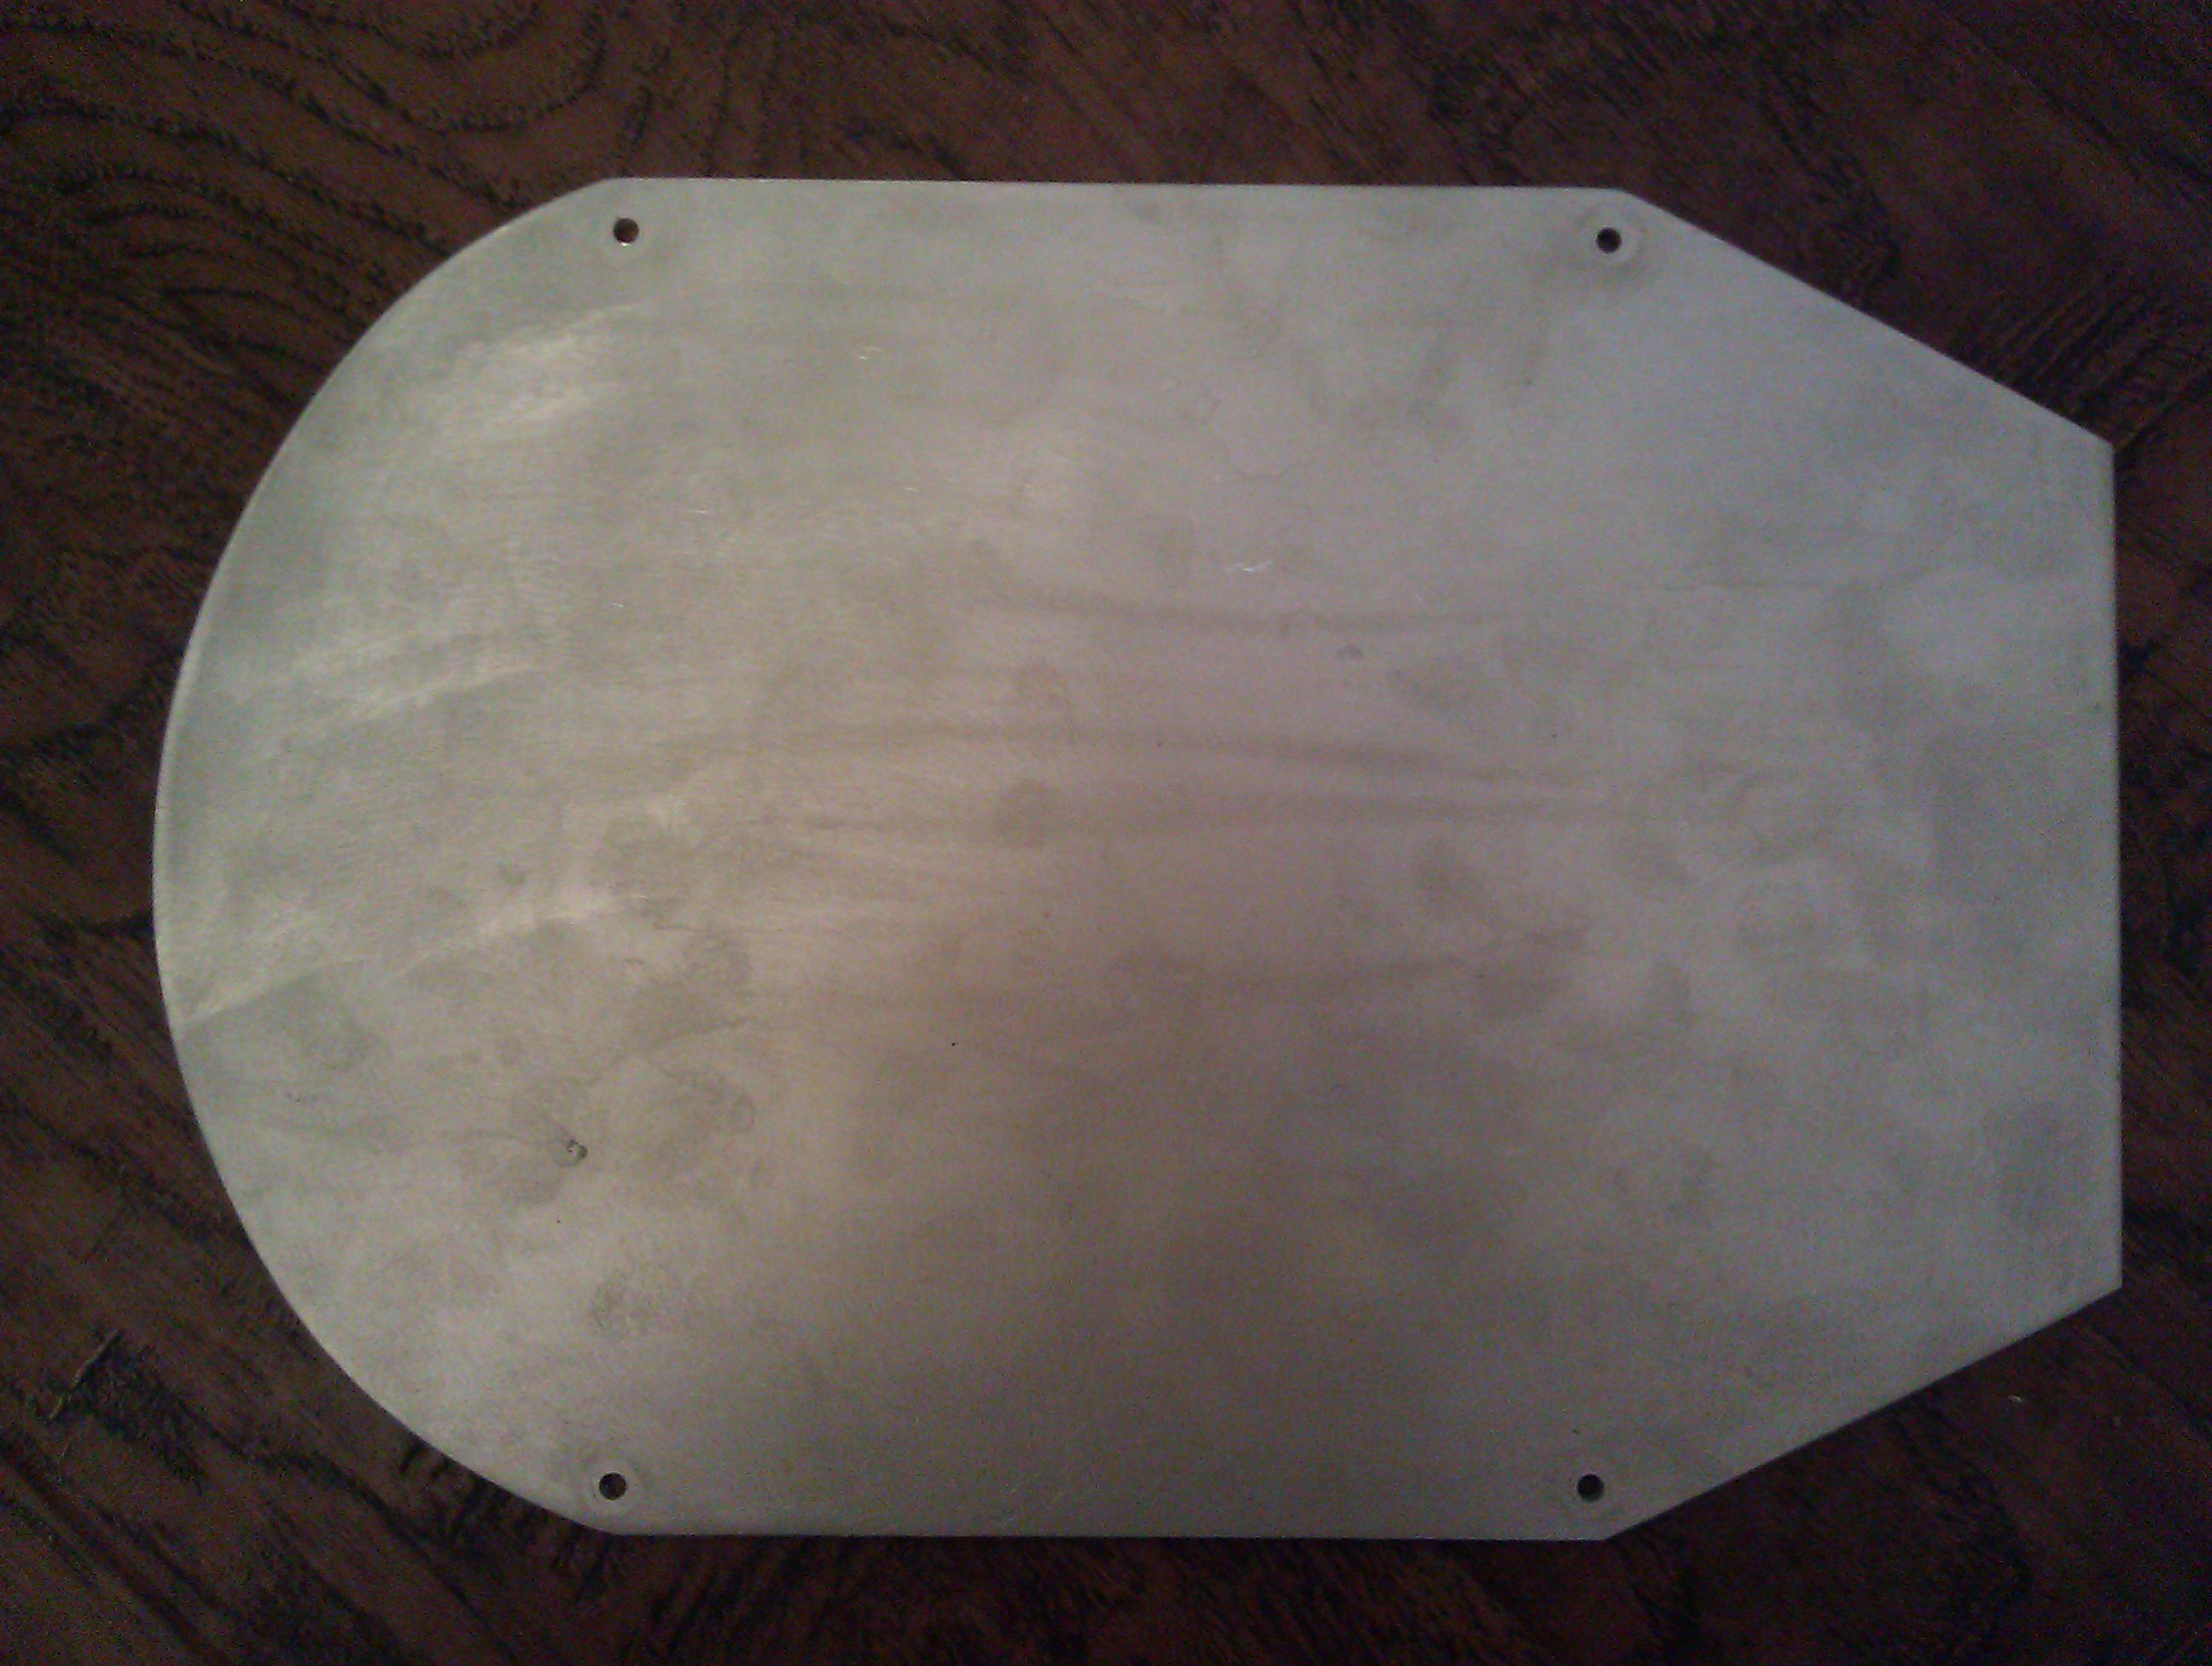
\includegraphics[width=3.0in]  {Images/alu-cut-2.jpg}
        \caption{Aluminium Sheet Cut}
        \label{Aluminium Sheet Cut}
\end{figure}
Next was to think about how to mount the motors to this aluminium base plate. After measuring the size of the stepper motors I bought to use as part of the robots drive system I also purchased a strip of aluminium to be cut and shaped into a motor mount to be attached on the underside of the baseplate.
\begin{figure}[H]
\centering
        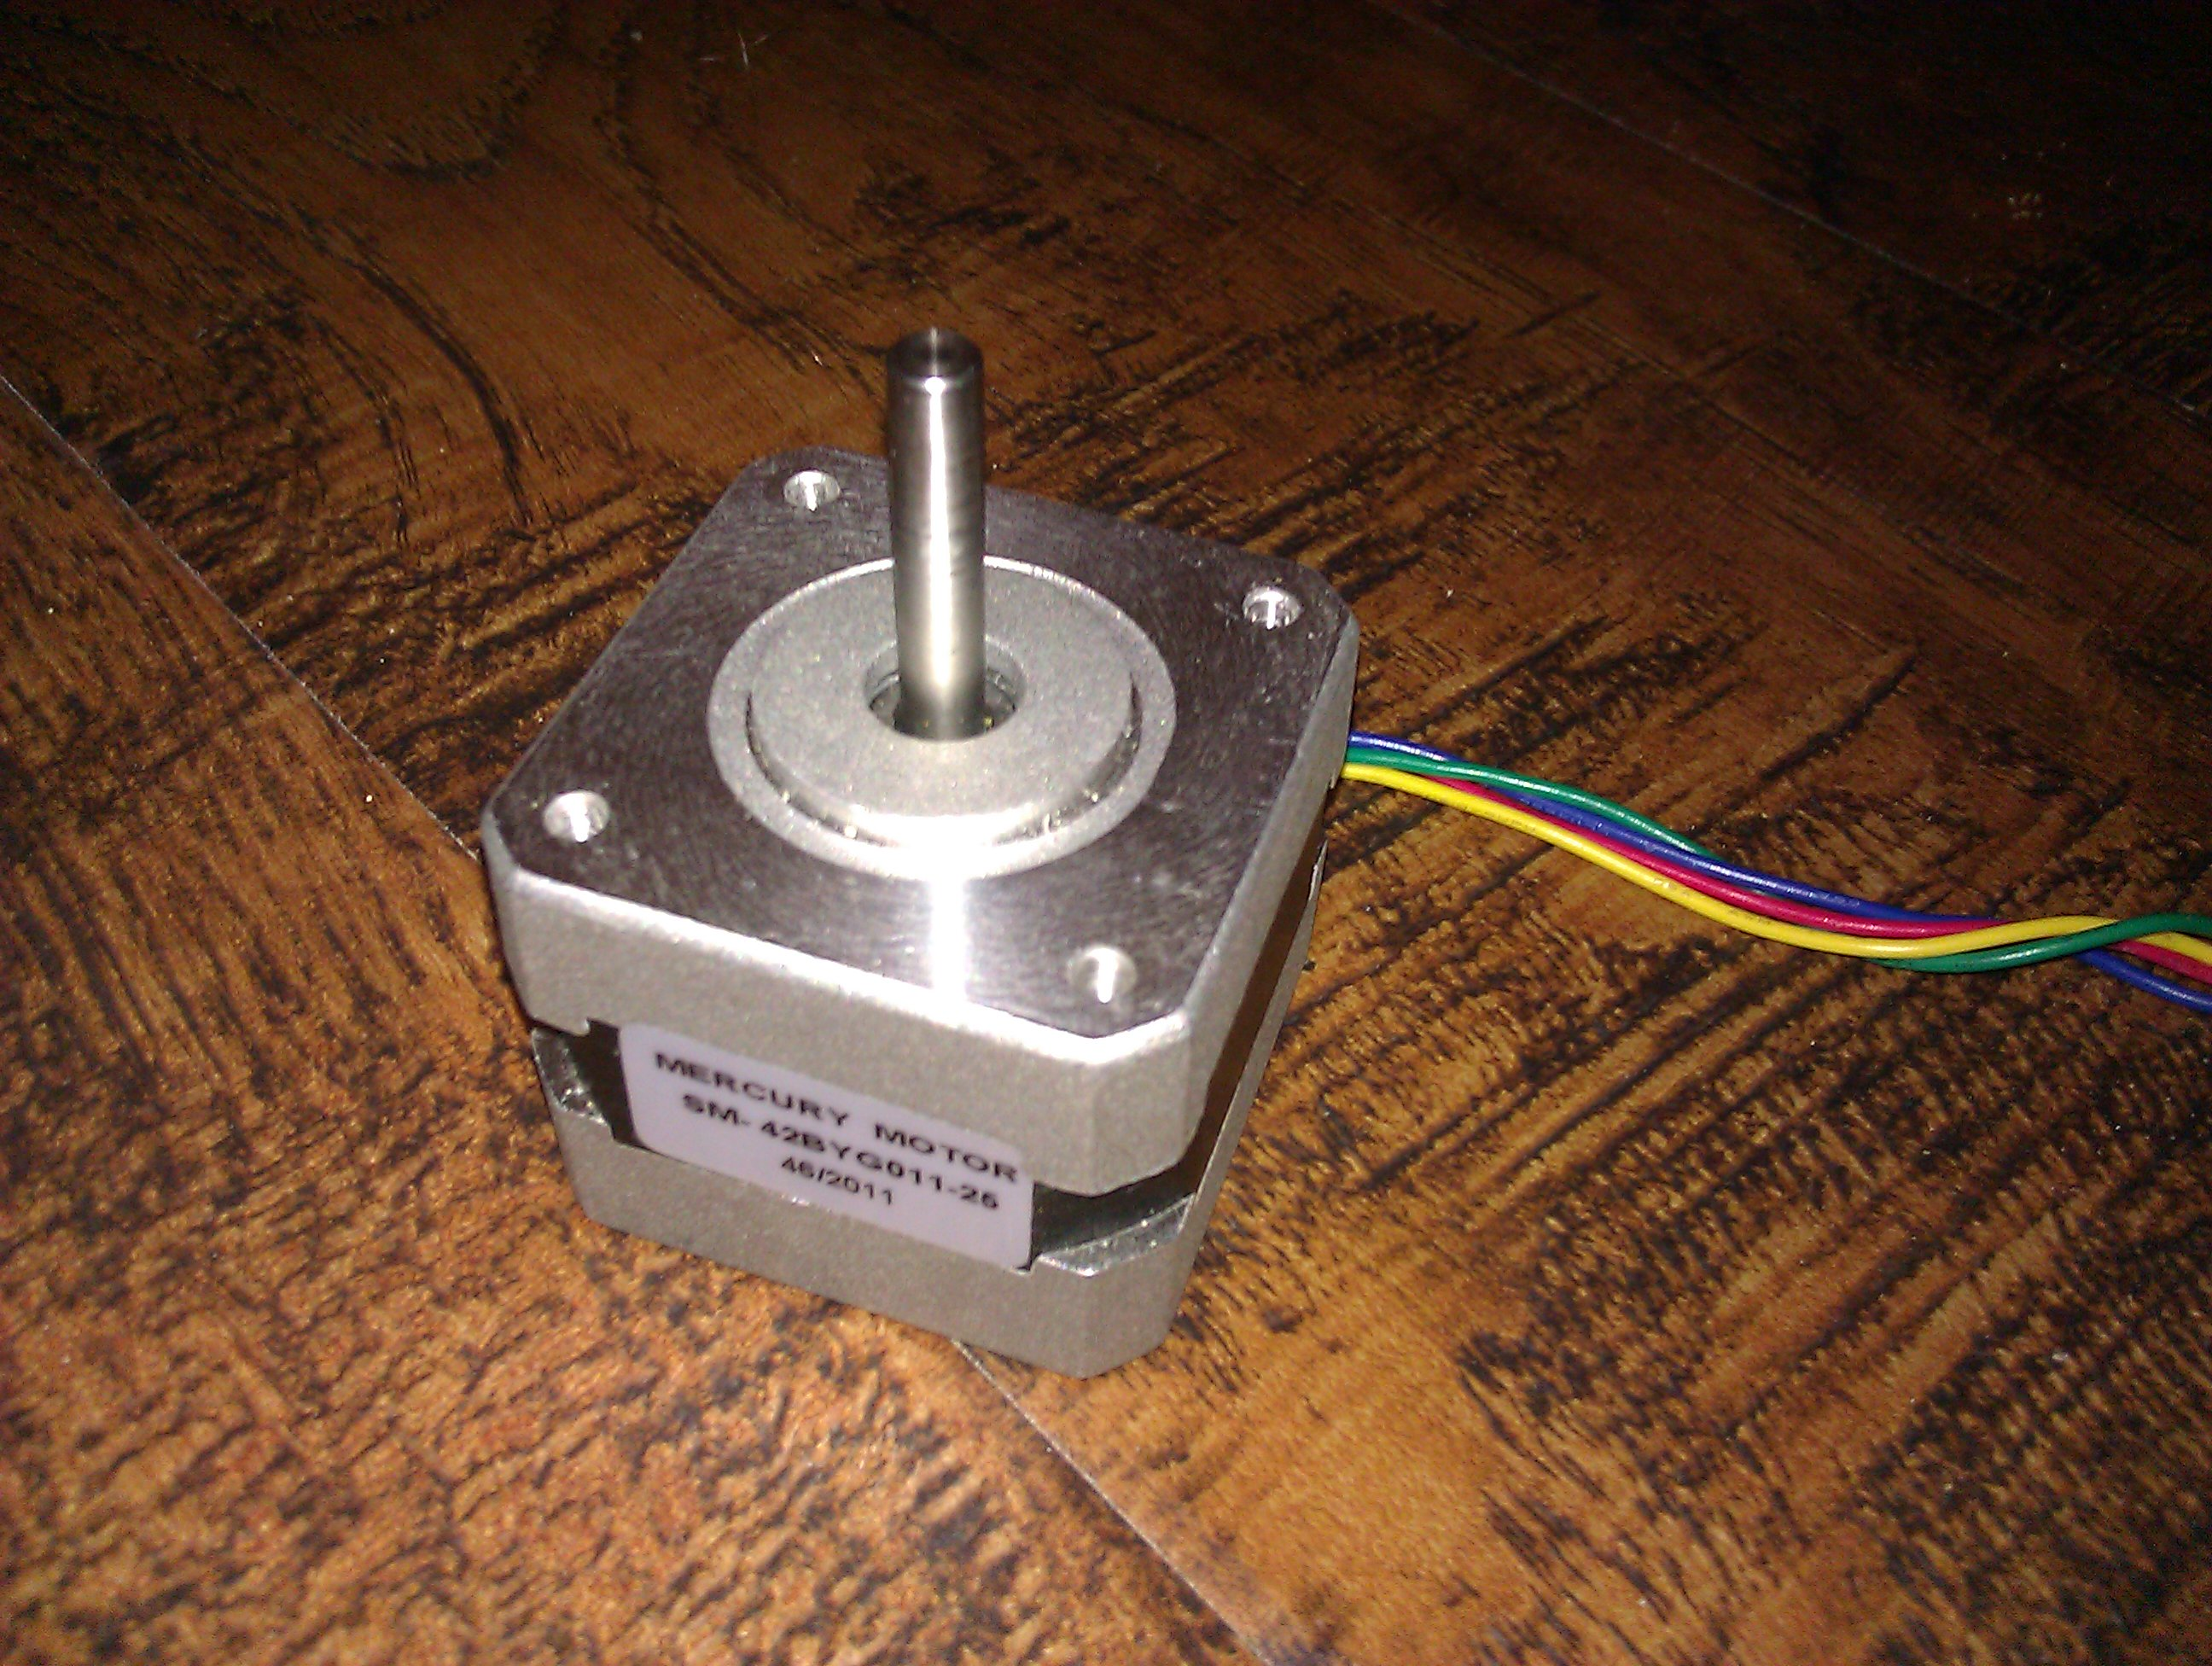
\includegraphics[width=3.0in]  {Images/small-stepper.jpg}
        \caption{Chosen Stepper Motor}
        \label{Chosen Stepper Motor}
\end{figure}
\begin{figure}[H]
\centering
        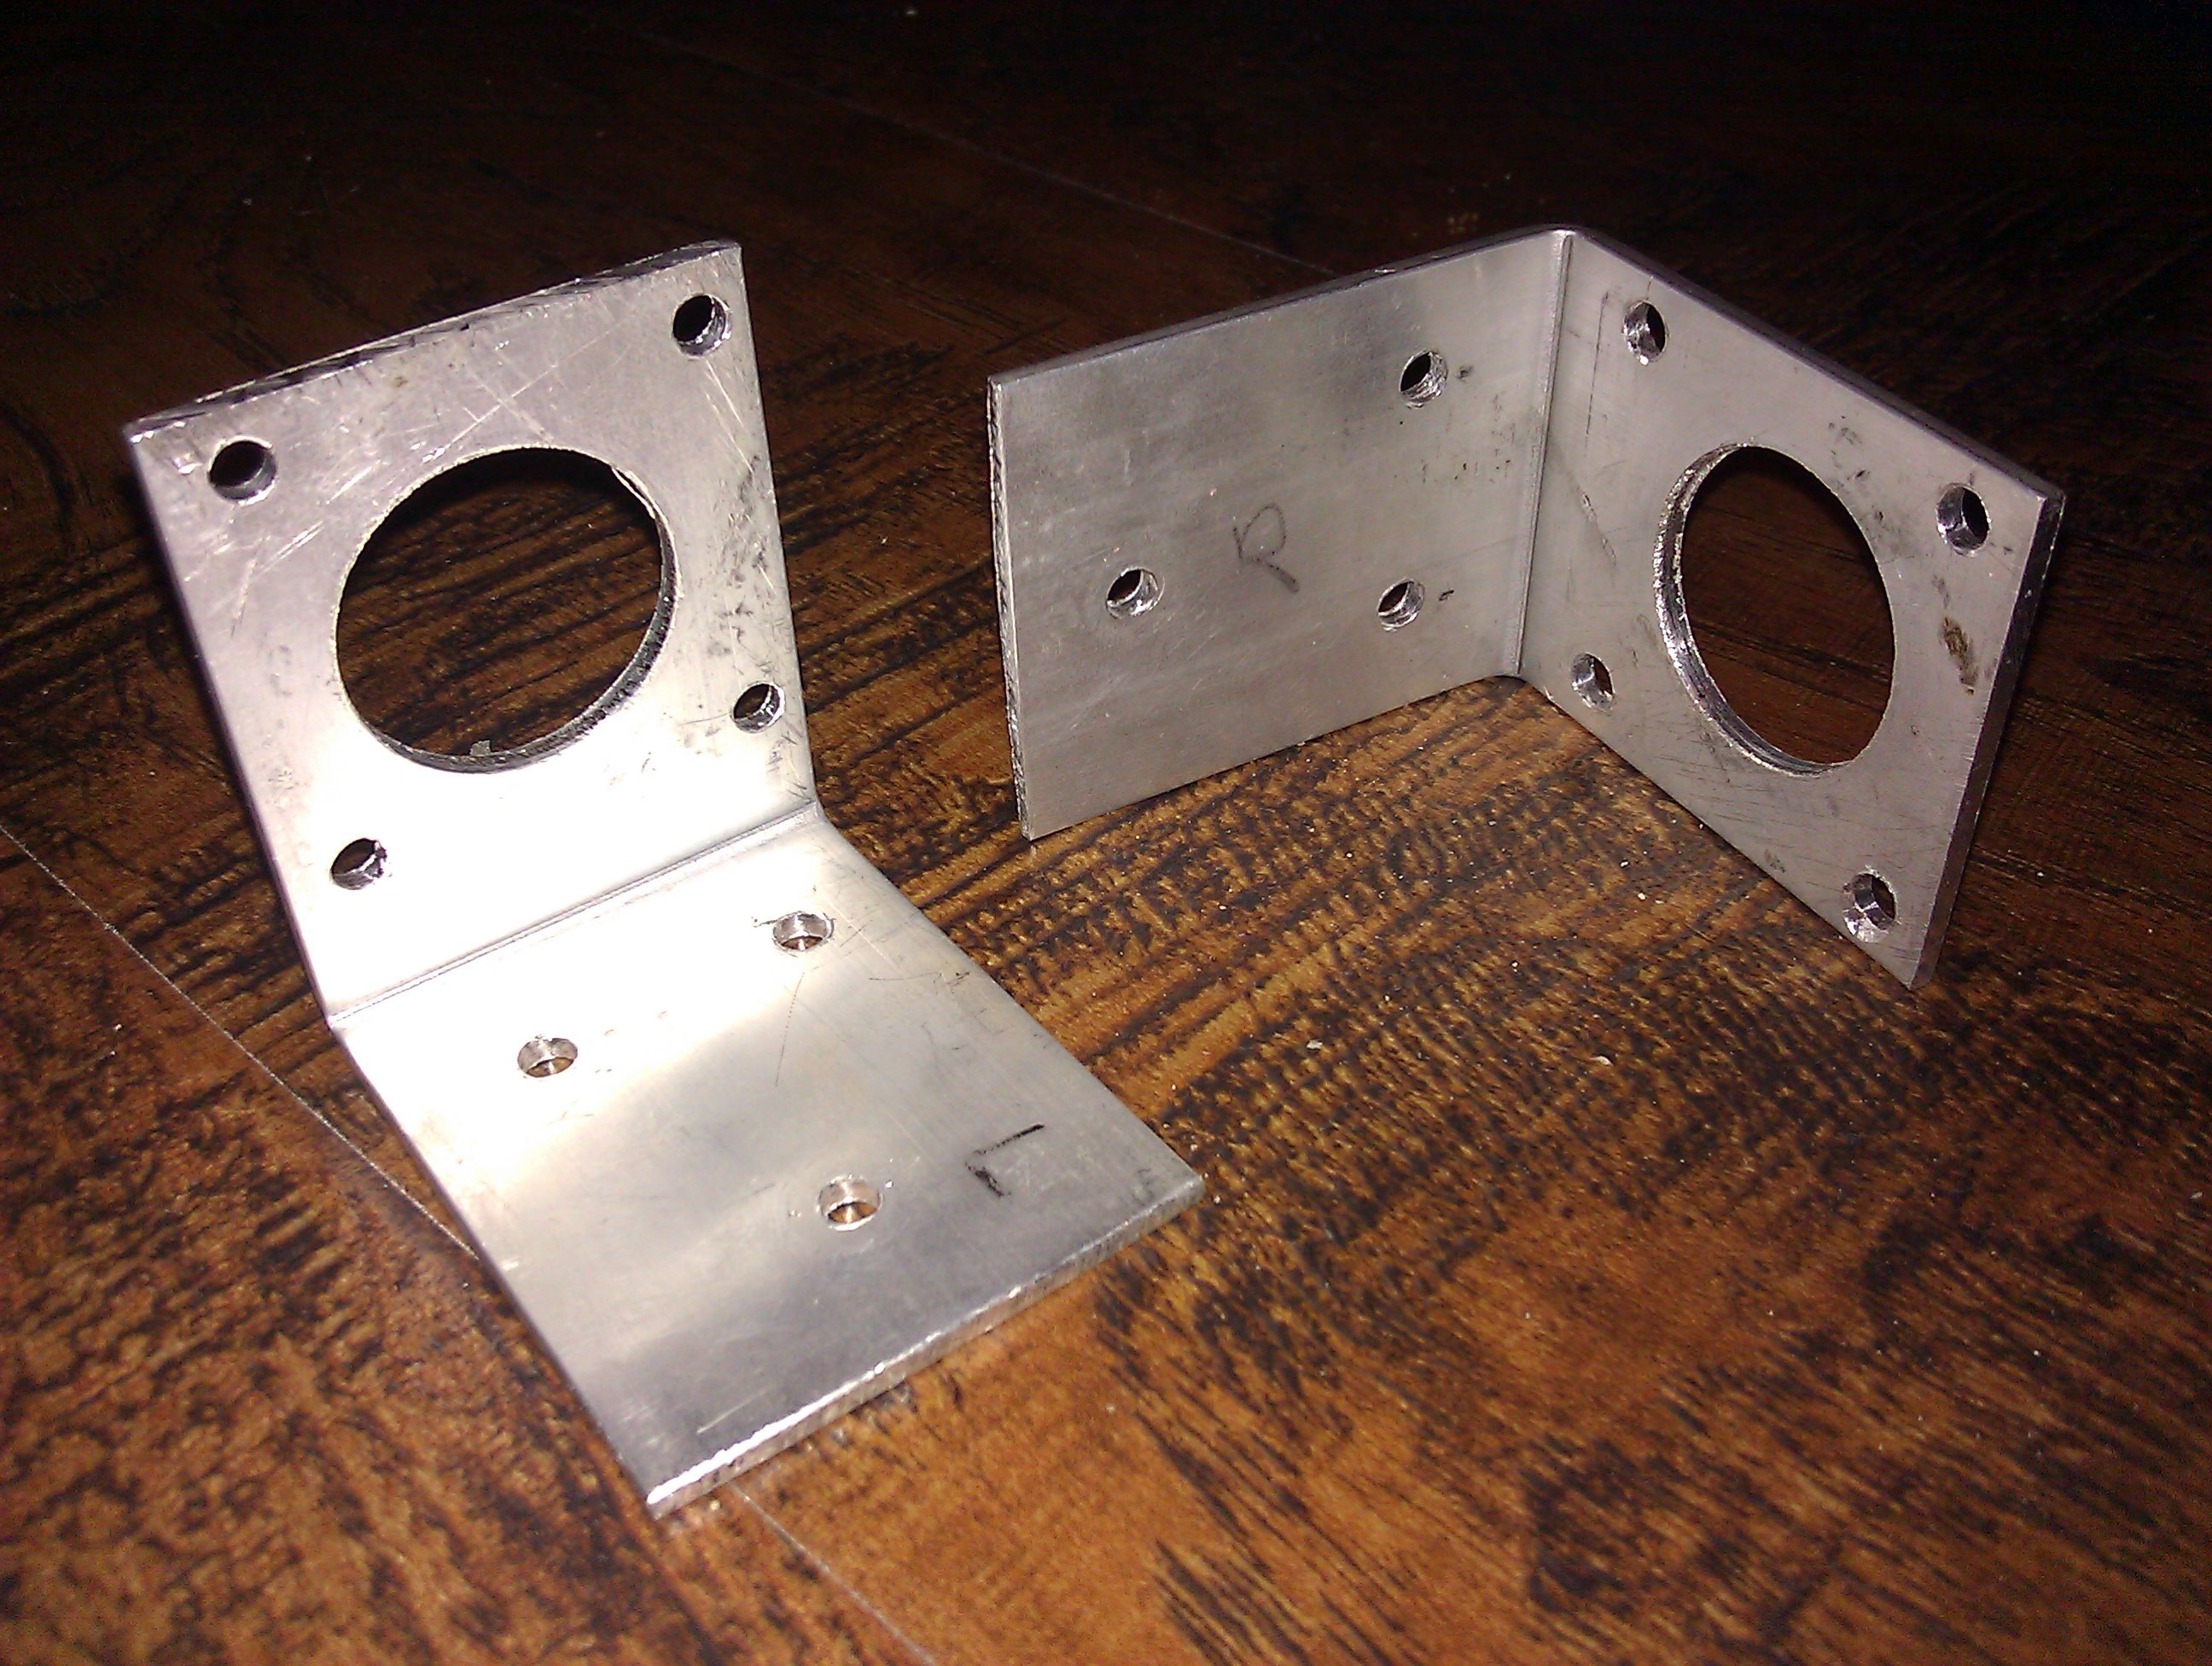
\includegraphics[width=3.0in]  {Images/motor-mount-1.jpg}
        \caption{Motor Mounts}
        \label{Motor Mounts}
\end{figure}
These mounts are just the cut strips of aluminium that have been bent so that they form a 90 degree angle and holes drilled through them to accommodate the motor drive shaft and for screw holes to attach these mounts to the baseplate.
\\Another alteration to the original design is the fact that I have chosen to use only two drive wheels instead of the four shown in the design document.  The reasoning for this was that it is easier to turn with just the two wheels as it will be able to almost turn on the spot rather than having to perform a multi directional turn, moving backwards and forwards turning a different direction for each just like how a driver would turn a car around in a tight space.  Also the kit used in the prototype only used two drive wheels with a caster wheel for stability and was in fact very stable, more than stable enough for this project and removes some complexity from the drive system.
\begin{figure}[H]
\centering
        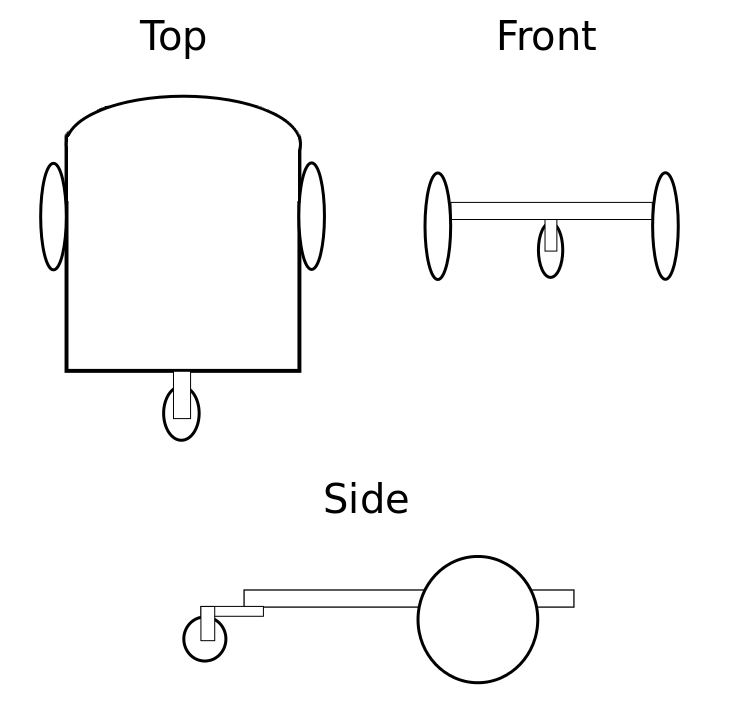
\includegraphics[width=4.0in]  {Images/second-design.png}
        \caption{Two Wheel Drive Design}
        \label{Two Wheel Drive Design}
\end{figure}
Now that the design has been reduced from four drive motors down to only two it will need some other wheels to keep the robot stable.  A single rear caster wheel worked well for the prototype and if I went with two rear stabilising wheels then the car turning in a tight space issue would still apply and because of this a single wheel has been chosen.
\\This wheel again has been mounted on a strip of aluminium bolted hanging over the rear end of the also aluminium baseplate.
\begin{figure}[H]
\centering
        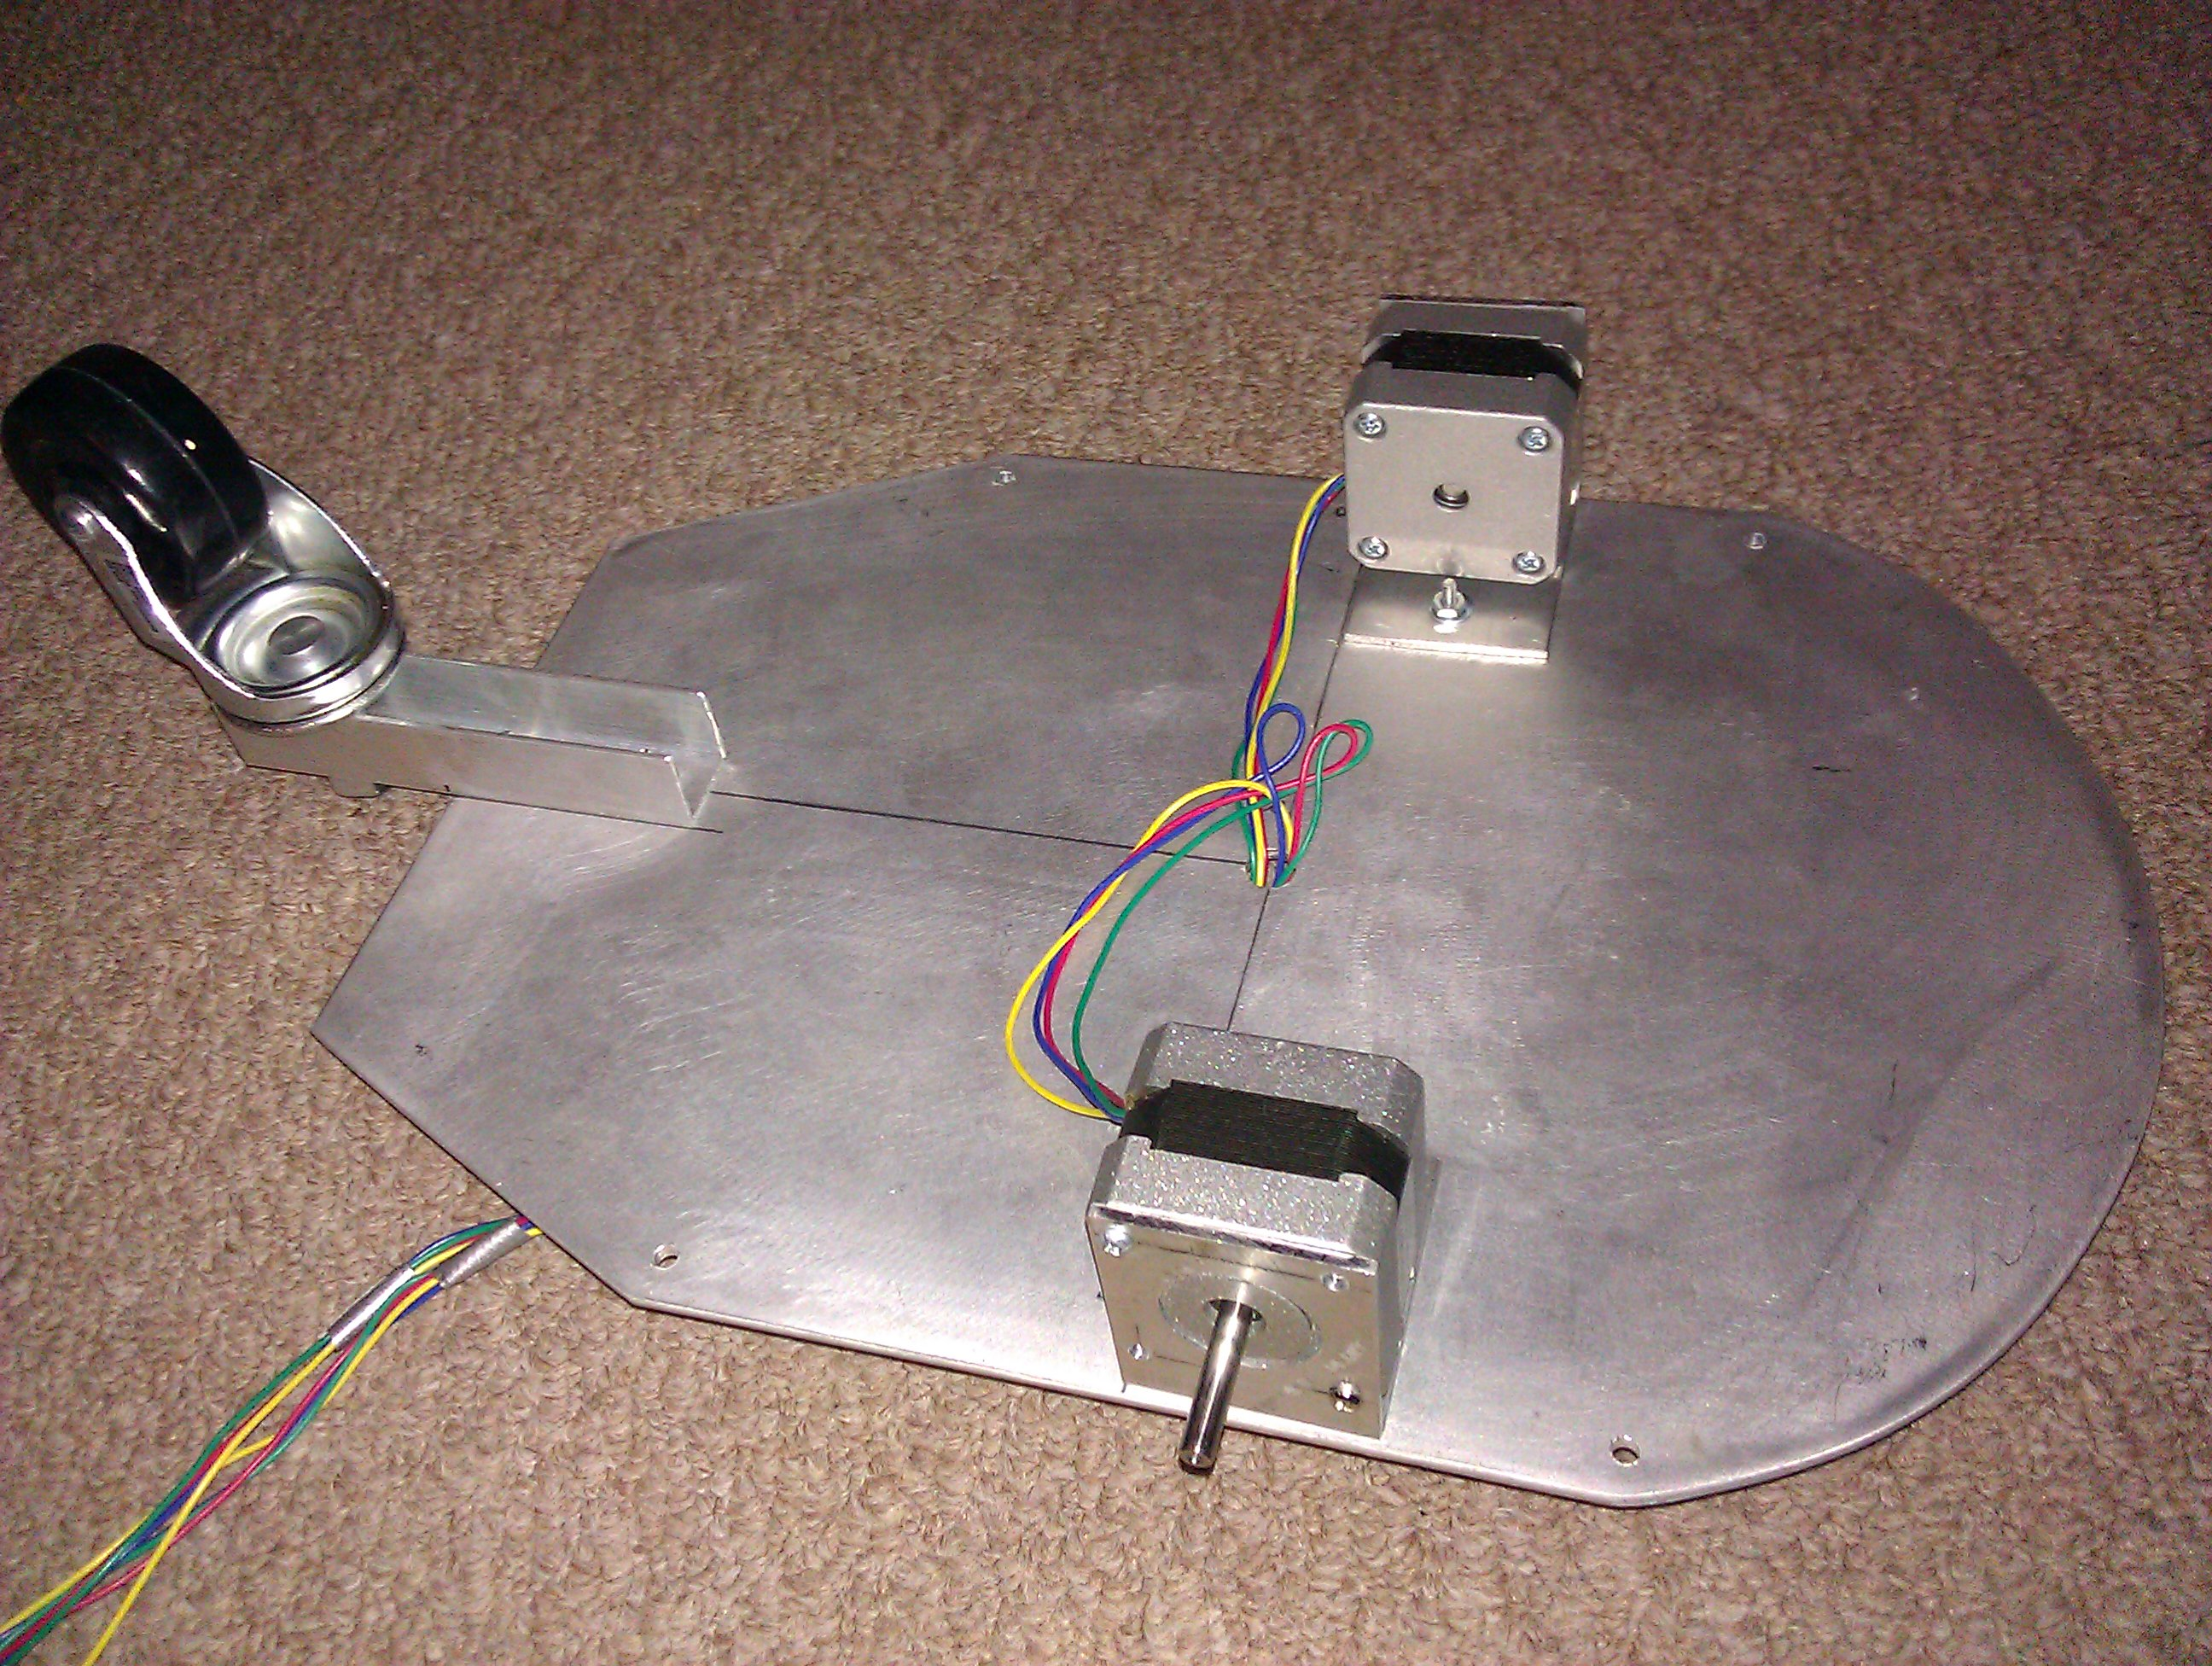
\includegraphics[width=3.0in]  {Images/baseplate-underside.jpg}
        \caption{Baseplate Underside}
        \label{Baseplate Underside}
\end{figure}
Next was to attach the stepper motors to the cut out motor mounting plates and attach the chosen off road wheels to them.  The wheels are attached to the motor shaft with the use of a hollow shaft attached to the wheel and a grub screw through that hollow shaft to clamp onto a flat edge that I cut into the motor shaft for grip.
\subsection{Manufacturing Parts}
Before starting this project I spent some time building a three dimensional printer.  This device is just like an ordinary printer but creates three dimensional physical objects.
\\An ordinary printer uses a print head to dispense ink onto a sheet or paper or card to leave a permanent mark on it which after a lot of small applications of the ink will build up letters or a picture.  A three dimensional printer works in a very similar way.  Plastic is fed into the print head where it is heated up above the melting point of whichever plastic is being used then extruded out onto a heated print bed.  While this melted plastic is being extruded the head is being moved around to draw out the shape of whatever is being printed.  This is currently still essentially two dimensional, what happens next is that once the first layer is finished with either the print head moves up or the print bed moves down and the next layer is started.  This is how this type of printer works, after the first layer is printed onto the heated bed, the next layer is printed on top of the previous one.  This process continues as many times as necessary until the layers are built up into the full object.
\\This process is very useful as it wastes no materials as it is an additive process as opposed to other computer aided manufacturing methods which are generally subtractive.  This means that other machines cut away excess off of a block of a selected material when this printer only adds material that is needed.
\\The reason I built this printer is to produce one off custom components for any project I might need such a capability.  Instead of trying to source the exact component I want of the right size and shape, or having to modify something else, the idea of just being able to create a three dimensional model on a computer of the object I want to create and then just be able to make it at a whim is a very attractive prospect.  These parts do not only have to be plastic, there are 3D printers can can even print metal, some of these parts are used in aircraft\cite{mitprint} and even formula one\cite{f1print} cars.  These parts were made using a power type 3D printer which uses the same concept as the printers available for consumer purchase but instead of extruding melted plastic from a heated nozzle they use an extremely fine powder which is dusted over the print area and melted in the correct areas with lasers.
\begin{figure}[H]
\centering
        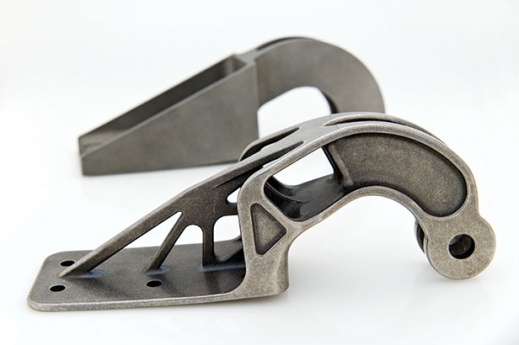
\includegraphics[width=4.0in]  {Images/print-aircraft.jpg}
        \caption{3D Printed Aircraft Part - technologyreview.com}
        \label{3D Printed Aircraft part}
\end{figure}

The printer I built had many printed components as parts of its own construction.  These parts were made out of a blue plastic. This printer was bought in kit form from a company called Felix Printers\cite{felix} in the Netherlands and took about a day to construct and a further day to configure and get working to an acceptable quality of parts produced by it.
\begin{figure}[H]
\centering
        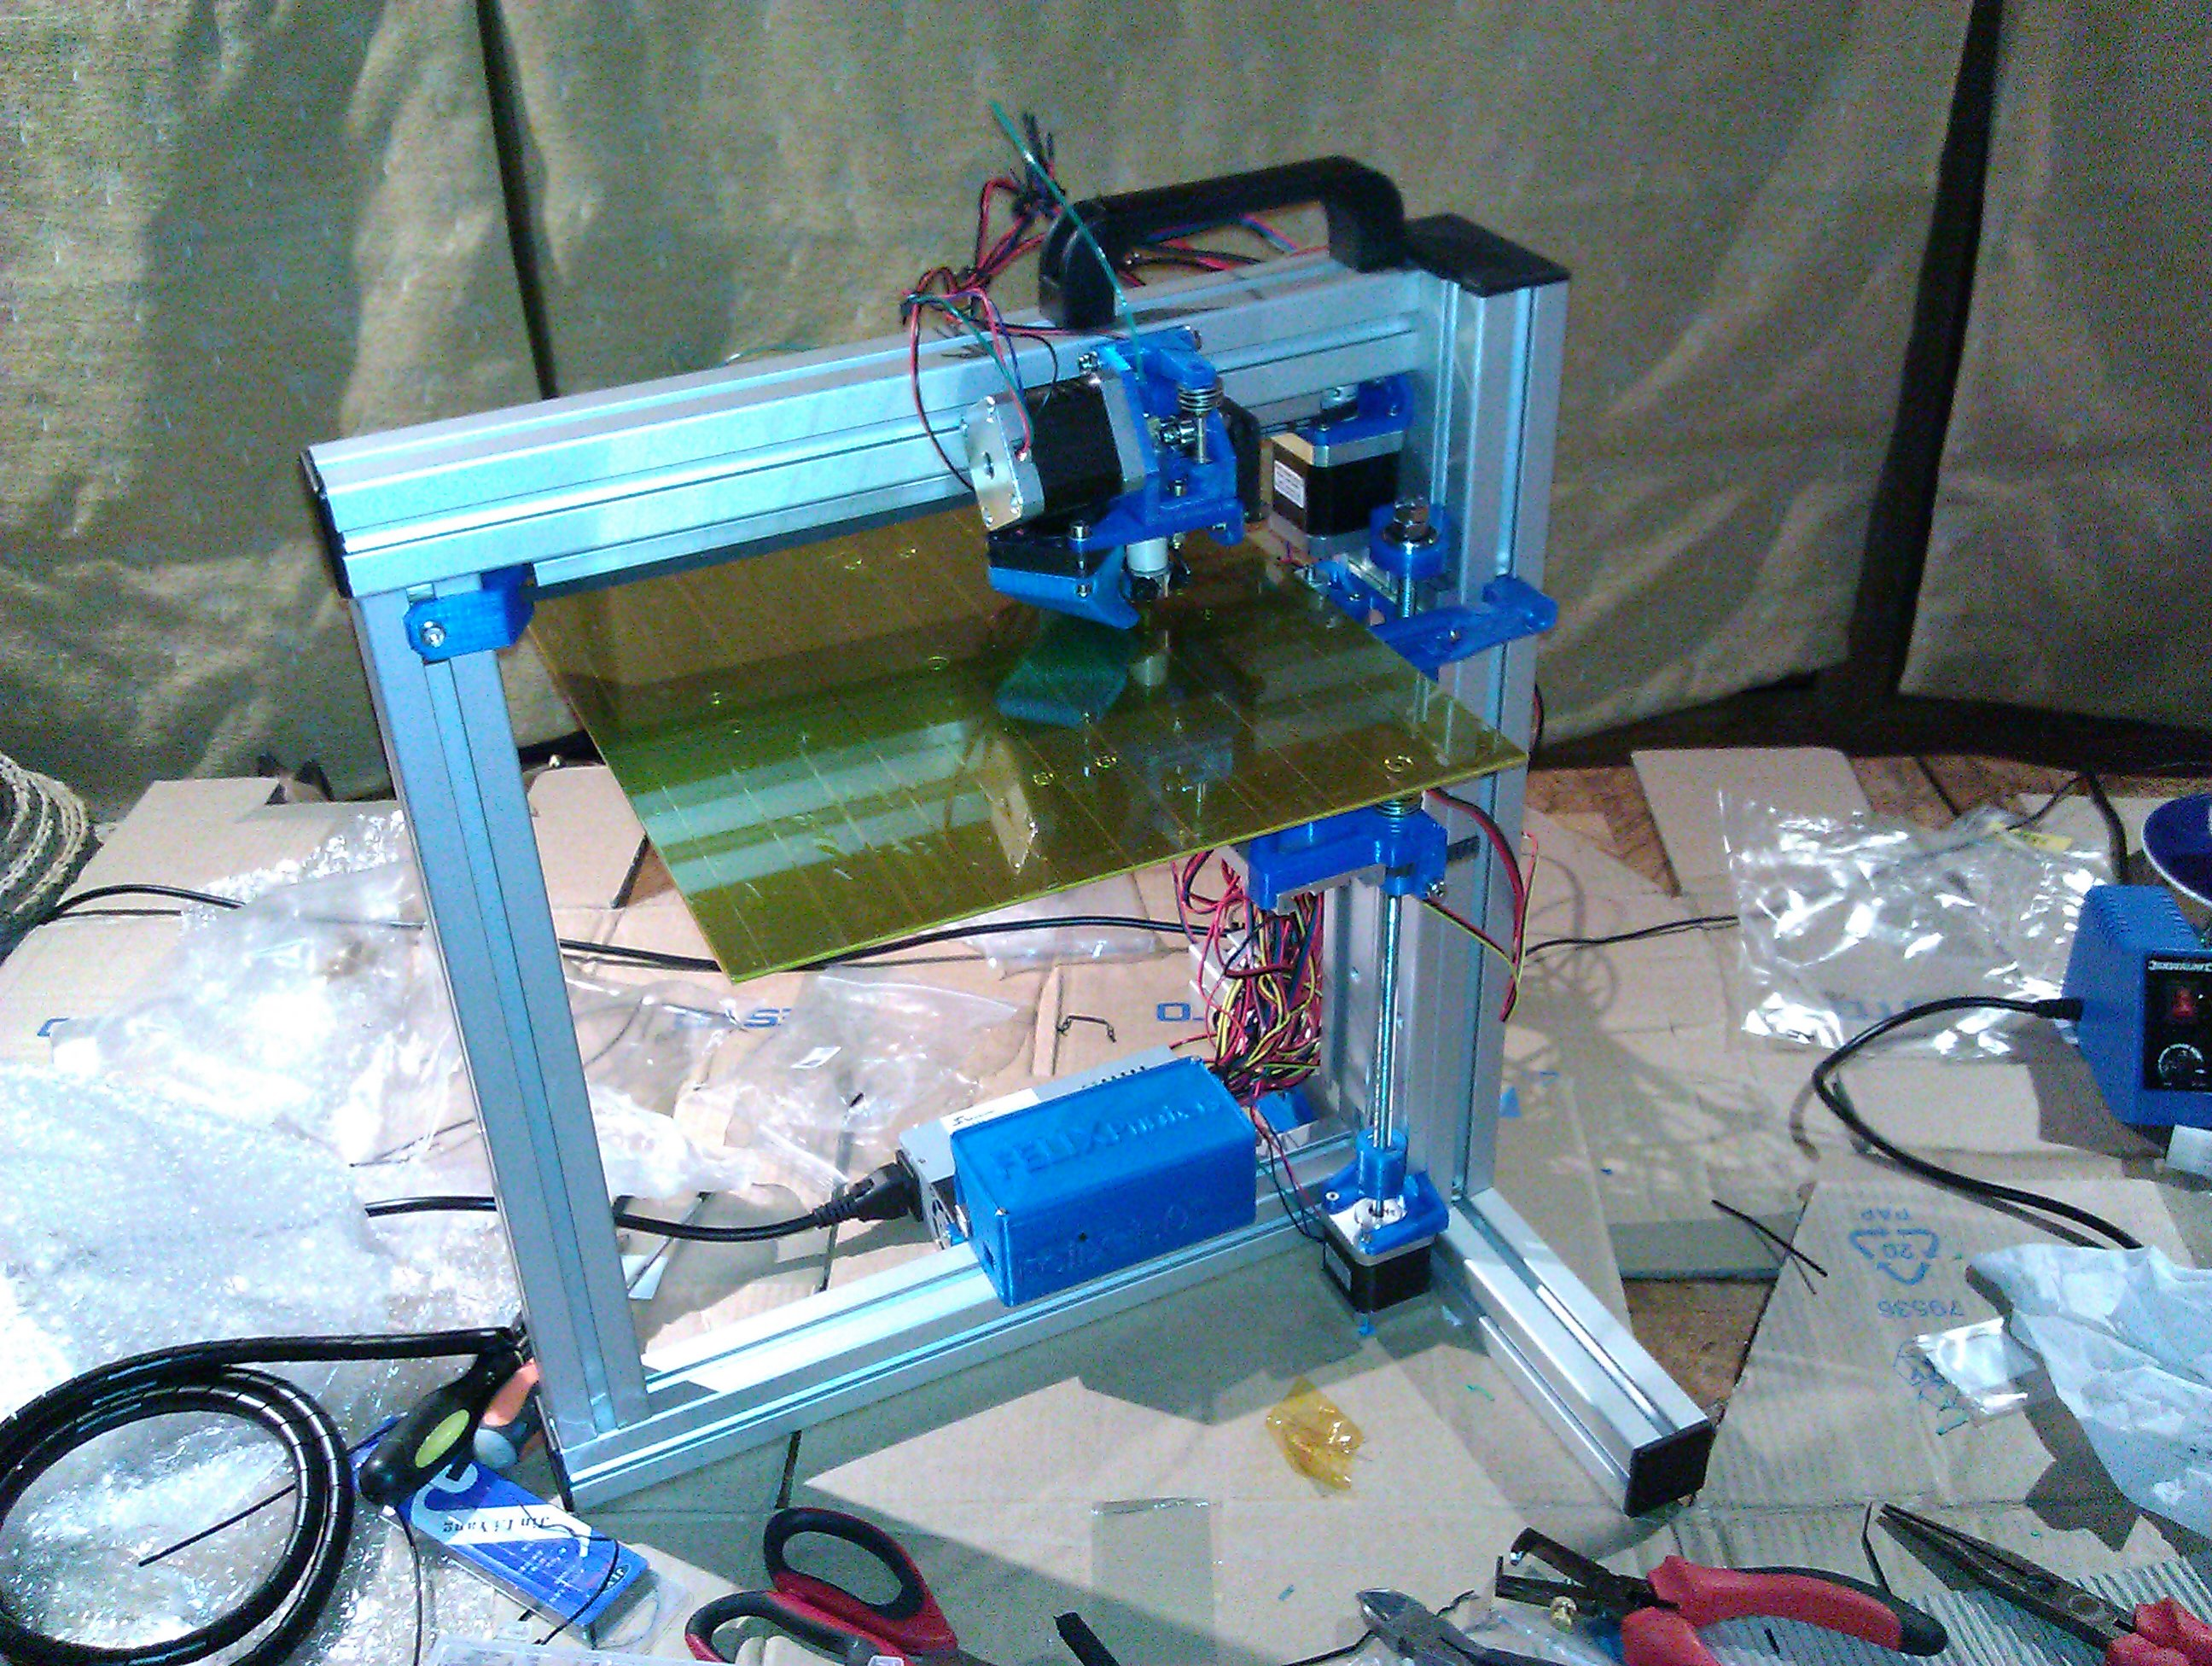
\includegraphics[width=5.0in]  {Images/printer.jpg}
        \caption{3D Printer}
        \label{3D Printer}
\end{figure}
The first component for the robot that I constructed with this printer is a mount for the microcontroller.  The mount is use to attach the component to the chassis and to insulate it from the metal base to avoid short circuits between varies part of the component and between it and other components that may also be mounted on the same base plate.  This mounting plate was constructed by the printer in less than half an hour and weighing under 25 grams and costing me less than 50 pence.
\begin{figure}[H]
\centering
        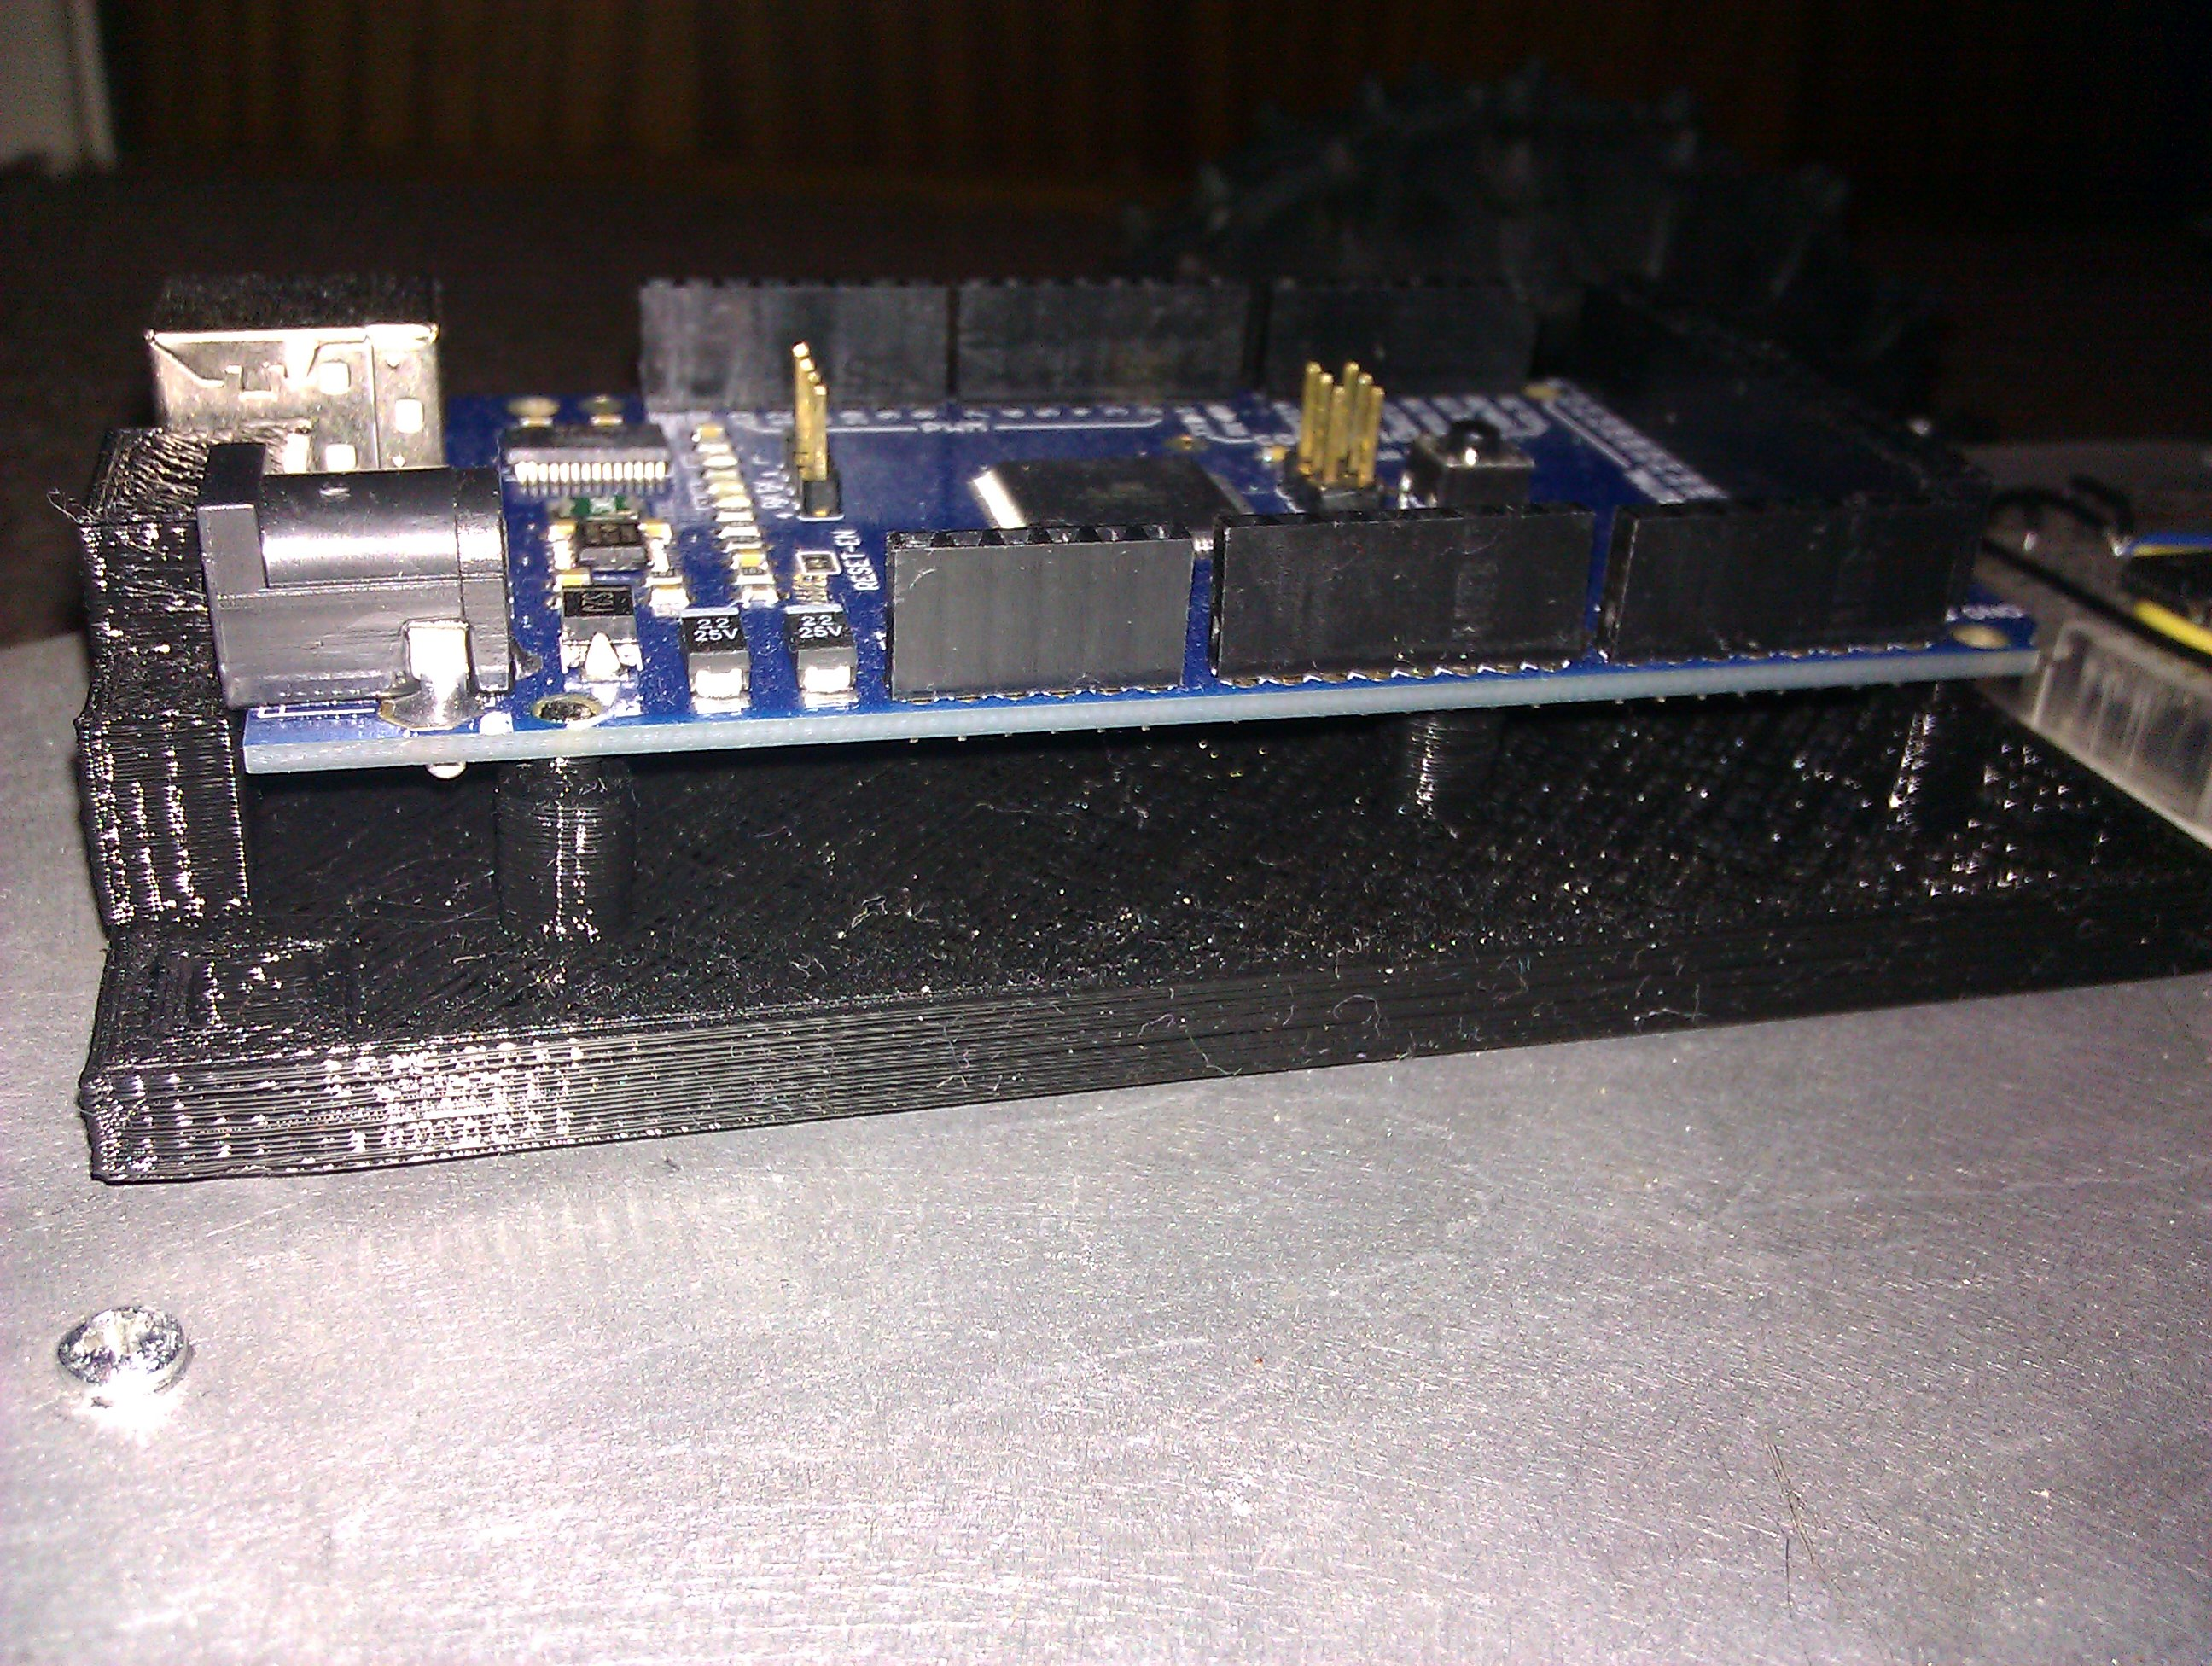
\includegraphics[width=5.0in]  {Images/printed-mount.jpg}
        \caption{Printed Mounting Plate}
        \label{Printed Mounting Plate}
\end{figure}
Eventually the printed mounting plate will be attached to the base plate with bolts but at this stage of development it is just help in place with adhesive tape.  There is a prototyping breadboard used for the h-bridge motor driver also fixed in place with the adhesive tape. With the drive wheels attached to the motors and mounted to the base plate, the rear caster wheel set in place, the Arduino microcontroller, the motor driver breadboard taped to the base plate and the motors wired up it was ready to write new motor control code as the prototype used a pair of DC motors and this iteration is using a pair of stepper motors.
\\To control a stepper motor there is a library to do so provided in the default set that the Arduino development environment supplies.  In the code which pins of the Arduino are being used to connect to the stepper motor has to be specified and then the library enables control of speed, direction and how many steps the motor is to turn.
\\\\It would be wise to note that at this point in the project the power source is not on board the robot as it had not yet arrived from the supplier, and so I was using a desktop computer power supply connected to a wall outlet and using long leads to link the robot power rails to the 12 volt line on the power supply.
\begin{figure}[H]
\centering
        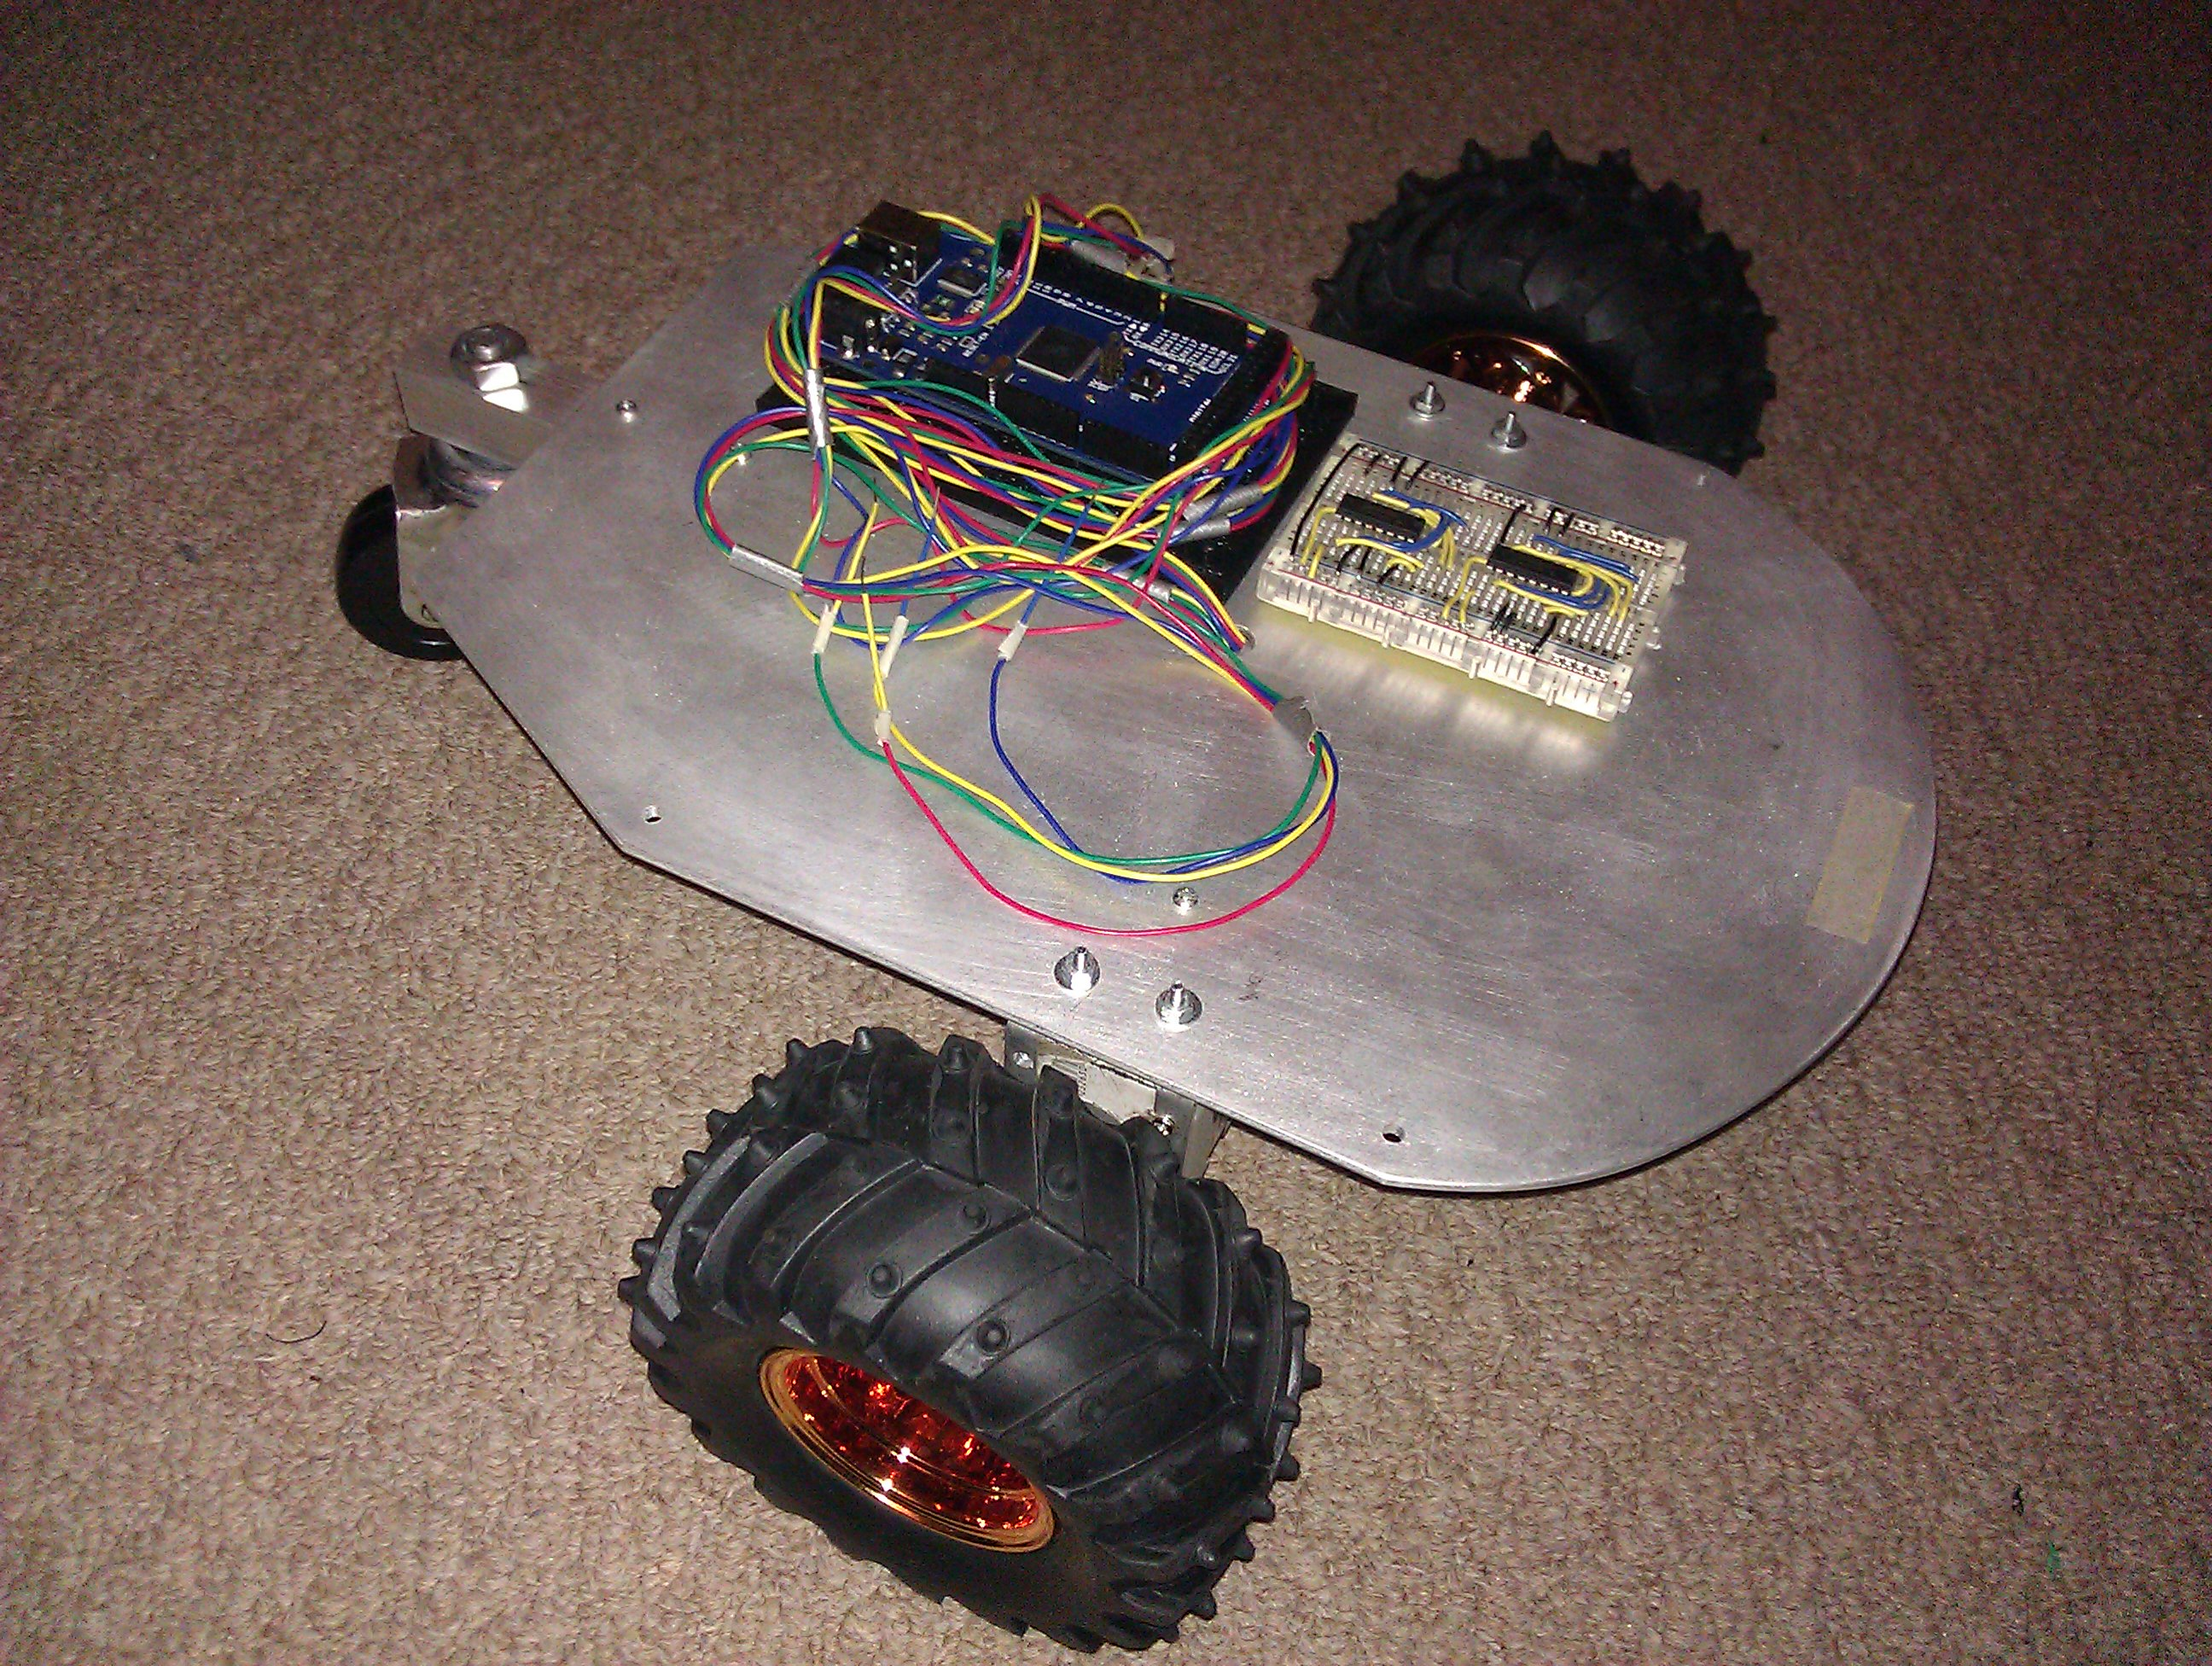
\includegraphics[width=5.0in]  {Images/tria-mkII.jpg}
        \caption{Completed MK-I}
        \label{Completed MK-I}
\end{figure}
\subsection{MK-I Evaluation}
It successfully drives itself forward in a straight line.  It does this very slowly and seems to struggle to do so with the motors seeming to jitter somewhat.  However it does move a set distance of one meter very reliably.  If the power supply has available and was fitted to the chassis I doubt the drive system would function as reliably as it is, or even move the robot at all.
\\The robot has a hard time turning reliably.  It does turn a significant amount but at the start of each turn it vibrates.  The vibrating is it struggling to shift it's weight but it does then start to turn.  This will be a problem when any additional weight is added on top of the chassis and not all of the components are fitted at this point.
\section{MK-II}
The power supply had still not arrived at this point and I had planned on building on the previous version by addressing the issue of the current drive system, but without the correct components of the right size and weight there was little point in pursuing this until the parts were available.  This iteration of the design will focus on the sensor system.
\\As the supplier I had placed my parts orders with had been having some unknown issues meeting their order commitments, at this point in the project I had still not received the bulk of the components that I had ordered.  This means that I still only had a single infrared sensor available to use.  There was no point in wasting time and waiting for these orders to be fulfilled and I moved straight onto using sonar as I had a pair of ultrasonic sensors.
\\These sensors are mounted by plugging their pins into a small prototyping breadboard each and connected to the microcontroller with jumper wires.  Instead of having the sensors facing directly forwards and due to the fact that only two were available I mounted them at an angle so each sensor can detect objects in a different region in front of the robot.  Unfortunately this means that anything small enough that is directly in front of the robot will not be detected by the sensors.
\begin{figure}[H]
\centering
        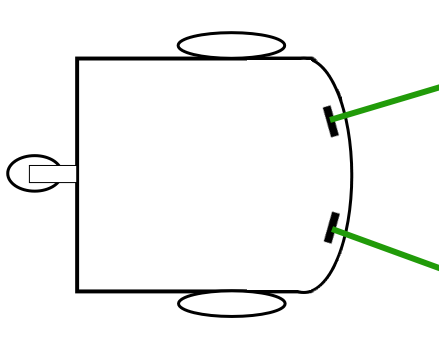
\includegraphics[width=2.0in]  {Images/sonar-placement.png}
        \caption{Sonar Configuration}
        \label{Sonar Configuration}
\end{figure}
This configuration would enable the robot to turn right or left depending on which sensor detected an object close to it.  Now that the robot could collect sensor data it was time to build the feedback interface that was previously mentioned so that I could check what the robot thinks its sensors are telling it without having to follow the robot around with a laptop and a long cable.
\subsection{Feedback Interface}
The fact that I wanted this to be small, compact and portable meant that using a breadboard to link the components together would not conform to that criteria and as such I connected the components directly together with solder and wires.
An Arduino Fio connected to the back of a 16 x 2 character liquid crystal display, with an xbee wireless module fitted into the modules slot on the Arduino unit as well as four buttons and a power switch glued to the base of the display for user interaction.  A small lithium polymer battery if help in place between the wireless module and the socket on the Arduino.  And the final component to make it all work is a small voltage step up unit to convert the Arduino's 3.3 volt output up to the 5 volts that the display needs to operate correctly.
\begin{figure}[H]
\centering
        \includegraphics[width=4.0in]  {Images/mobile-board.png}
        \caption{Feedback Interface}
        \label{Feedback Interface}
\end{figure}
This device just receives information sent from the robot about the values the sonar sensors are providing.
Each line of the display shows what distance each sensor thinks an object is away from itself.  I had written a small menu system on the device so that the user can check how long it has been running for, what the current sensor readings are and to even be able to manually control the drive system of the robot.
With the purpose of the device being that or portability I decided it needed to not be difficult to hold, as it was at this point because of the electronics being exposed.  It was then sewn into a glove so that it could be used hands free.  Having it inside a glove also protected the electronics from being interfered with.
\begin{figure}[H]
\centering
        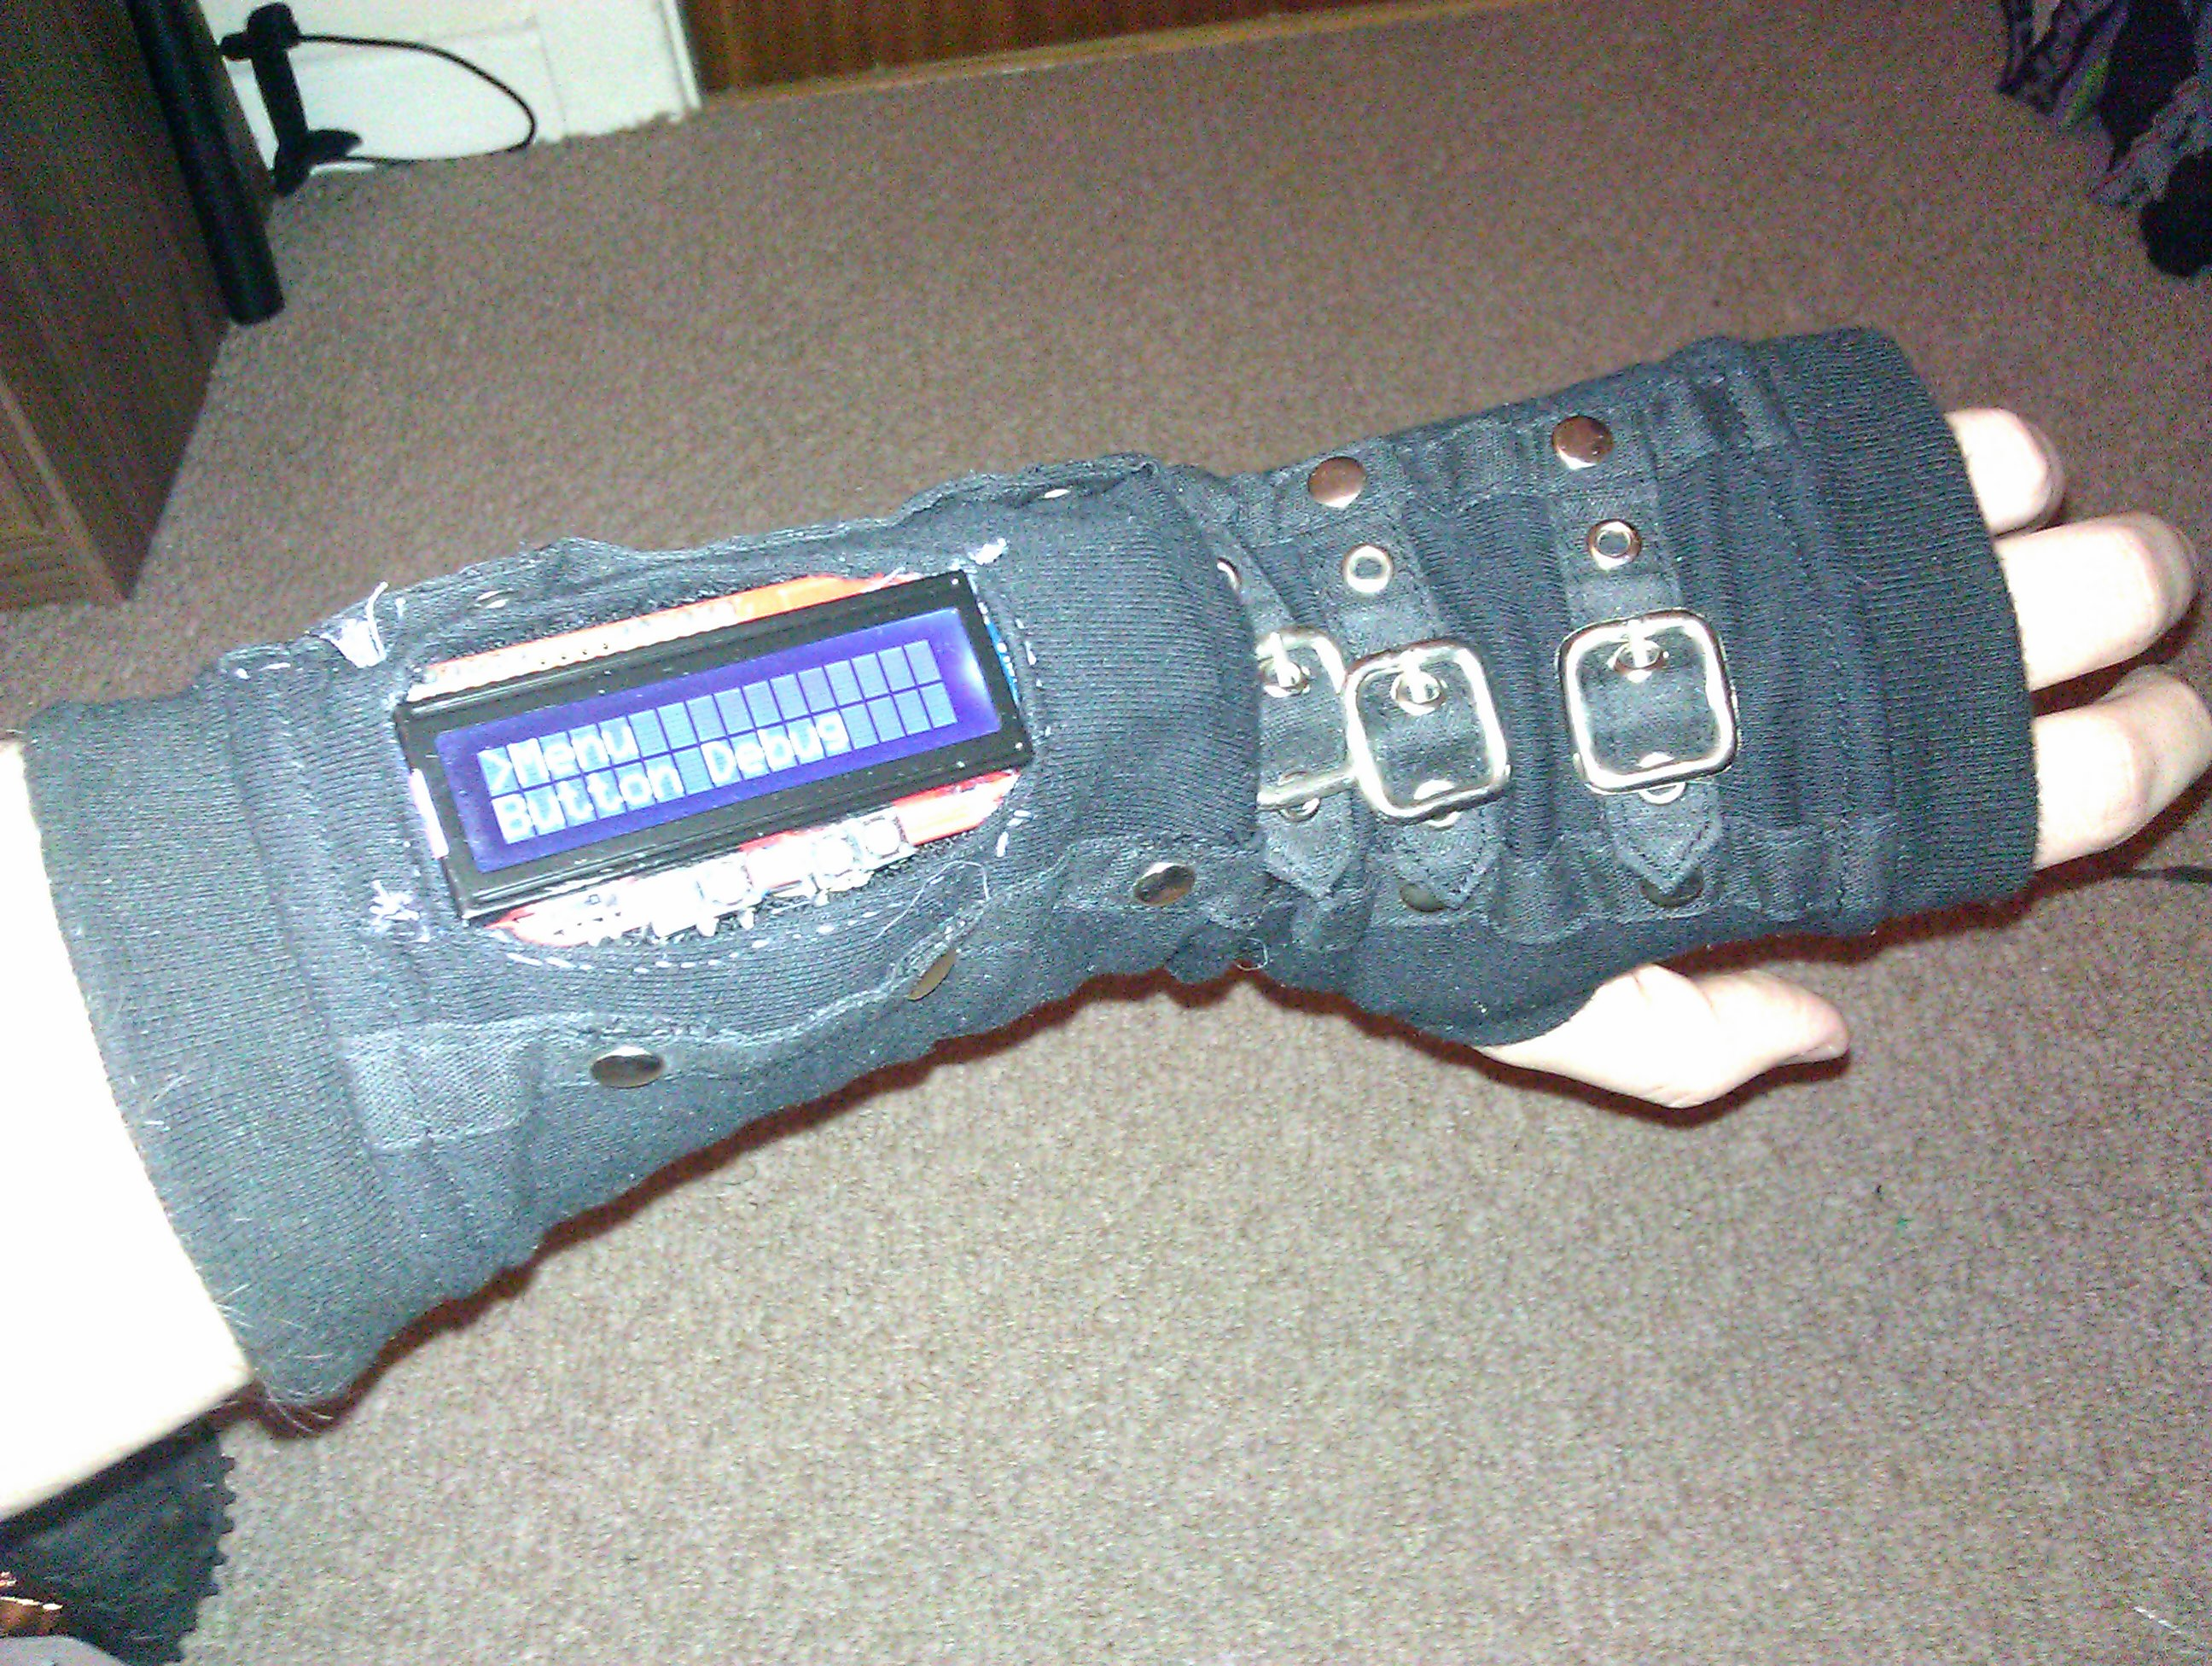
\includegraphics[width=4.0in]  {Images/wrist-device.jpg}
        \caption{Wrist Device}
        \label{Wrist Device}
\end{figure}
\subsection{MK-II Evaluation}
At this point the robot does move, but very slowly and with some difficulty, this is an issue that still needed solving. The robot can also detect if an object is in front of either sonar sensor.
\\The next step to improve on this iteration would be to enable the robot to turn to avoid an object that it has detected.
\section{MK-III}
This iteration was a short one due to the fact that the ordered parts had still not arrived from the supplier there was not much that could be done.  The only changed made to this version was in the software.  These changes were adding code that enabled the robot to change direction when approaching an obstacle.
First was to decide on a threshold value for when to trigger the robots decision to turn.  This was accomplished via trial and error, where I would set a default value and see if the robot actually avoided the obstruction.  This default value was the distance from the center of the robot to the outer edge of the wheel, the logic being that this is the minimum amount of space the robot would need to be able to turn in.
\\This turned out to not be enough due to how the robot struggles to move normally and when turning it has a harder time moving when turning.  The robot does not turn enough and drives at an angle into the obstacle it is trying to avoid.
\\I just increased the threshold to make the robot try to turn when it is much further away from the detected obstacle.
\subsection{MK-III Evaluation}
The MK-III iteration has highlighted the fact that the project could not move much further forwards until the rest of the ordered parts have arrived.
\\There is still the issue with the drive system not being strong enough to move the weight of the entire robot.
\\The other issue with the current iteration is that the sensor threshold had been calibrated to accommodate for the lack of power in the drive system and as such it tried to avoid objects too far away.  This can make the robot miss gaps that are big enough to easily fit through.
\begin{figure}[H]
\centering
        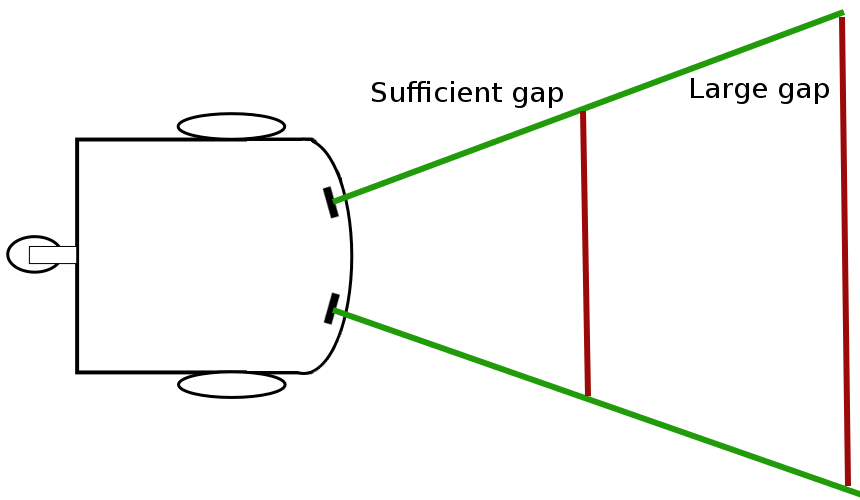
\includegraphics[width=4.0in]  {Images/sonar-range.png}
        \caption{Sonar Range Gap}
        \label{Sonar Range Gap}
\end{figure}
When the drive system is strong enough to make tighter turns the sonar range threshold can be re-calibrated to a much shorter distance and allow the robot to move inside much tighter spaces.

\section{MK-IV}
The supplier had fulfilled their orders by this time and I now had the parts that I needed.  After mounting the power supply onto the chassis in the form of a lead acid battery and some adhesive tape, I tested if the current drive system could still move with the extra weight.
\\As it struggled to move when the power source was not on-board it was unlikely to cope any better when a heavy lead acid battery is added to the payload.  The robot no longer moves under it's own power apart from vibrating violently as the motors try to turn the wheels.
\\The stepper motors I previously bought for the project did not have enough torque to move the weight of the full payload.  When this first came apparent I ordered a pair of stepper motors with a much higher holding torque rating of 125 oz.inch.
\\These new motors are much bigger than the old ones which required me to make new motor mounts.  I made these mounts out of the excess aluminium strips I had left after making the first pair of motor mounts and designed them to use the same mounting holes as the first pair of mounts.
\begin{figure}[H]
\centering
        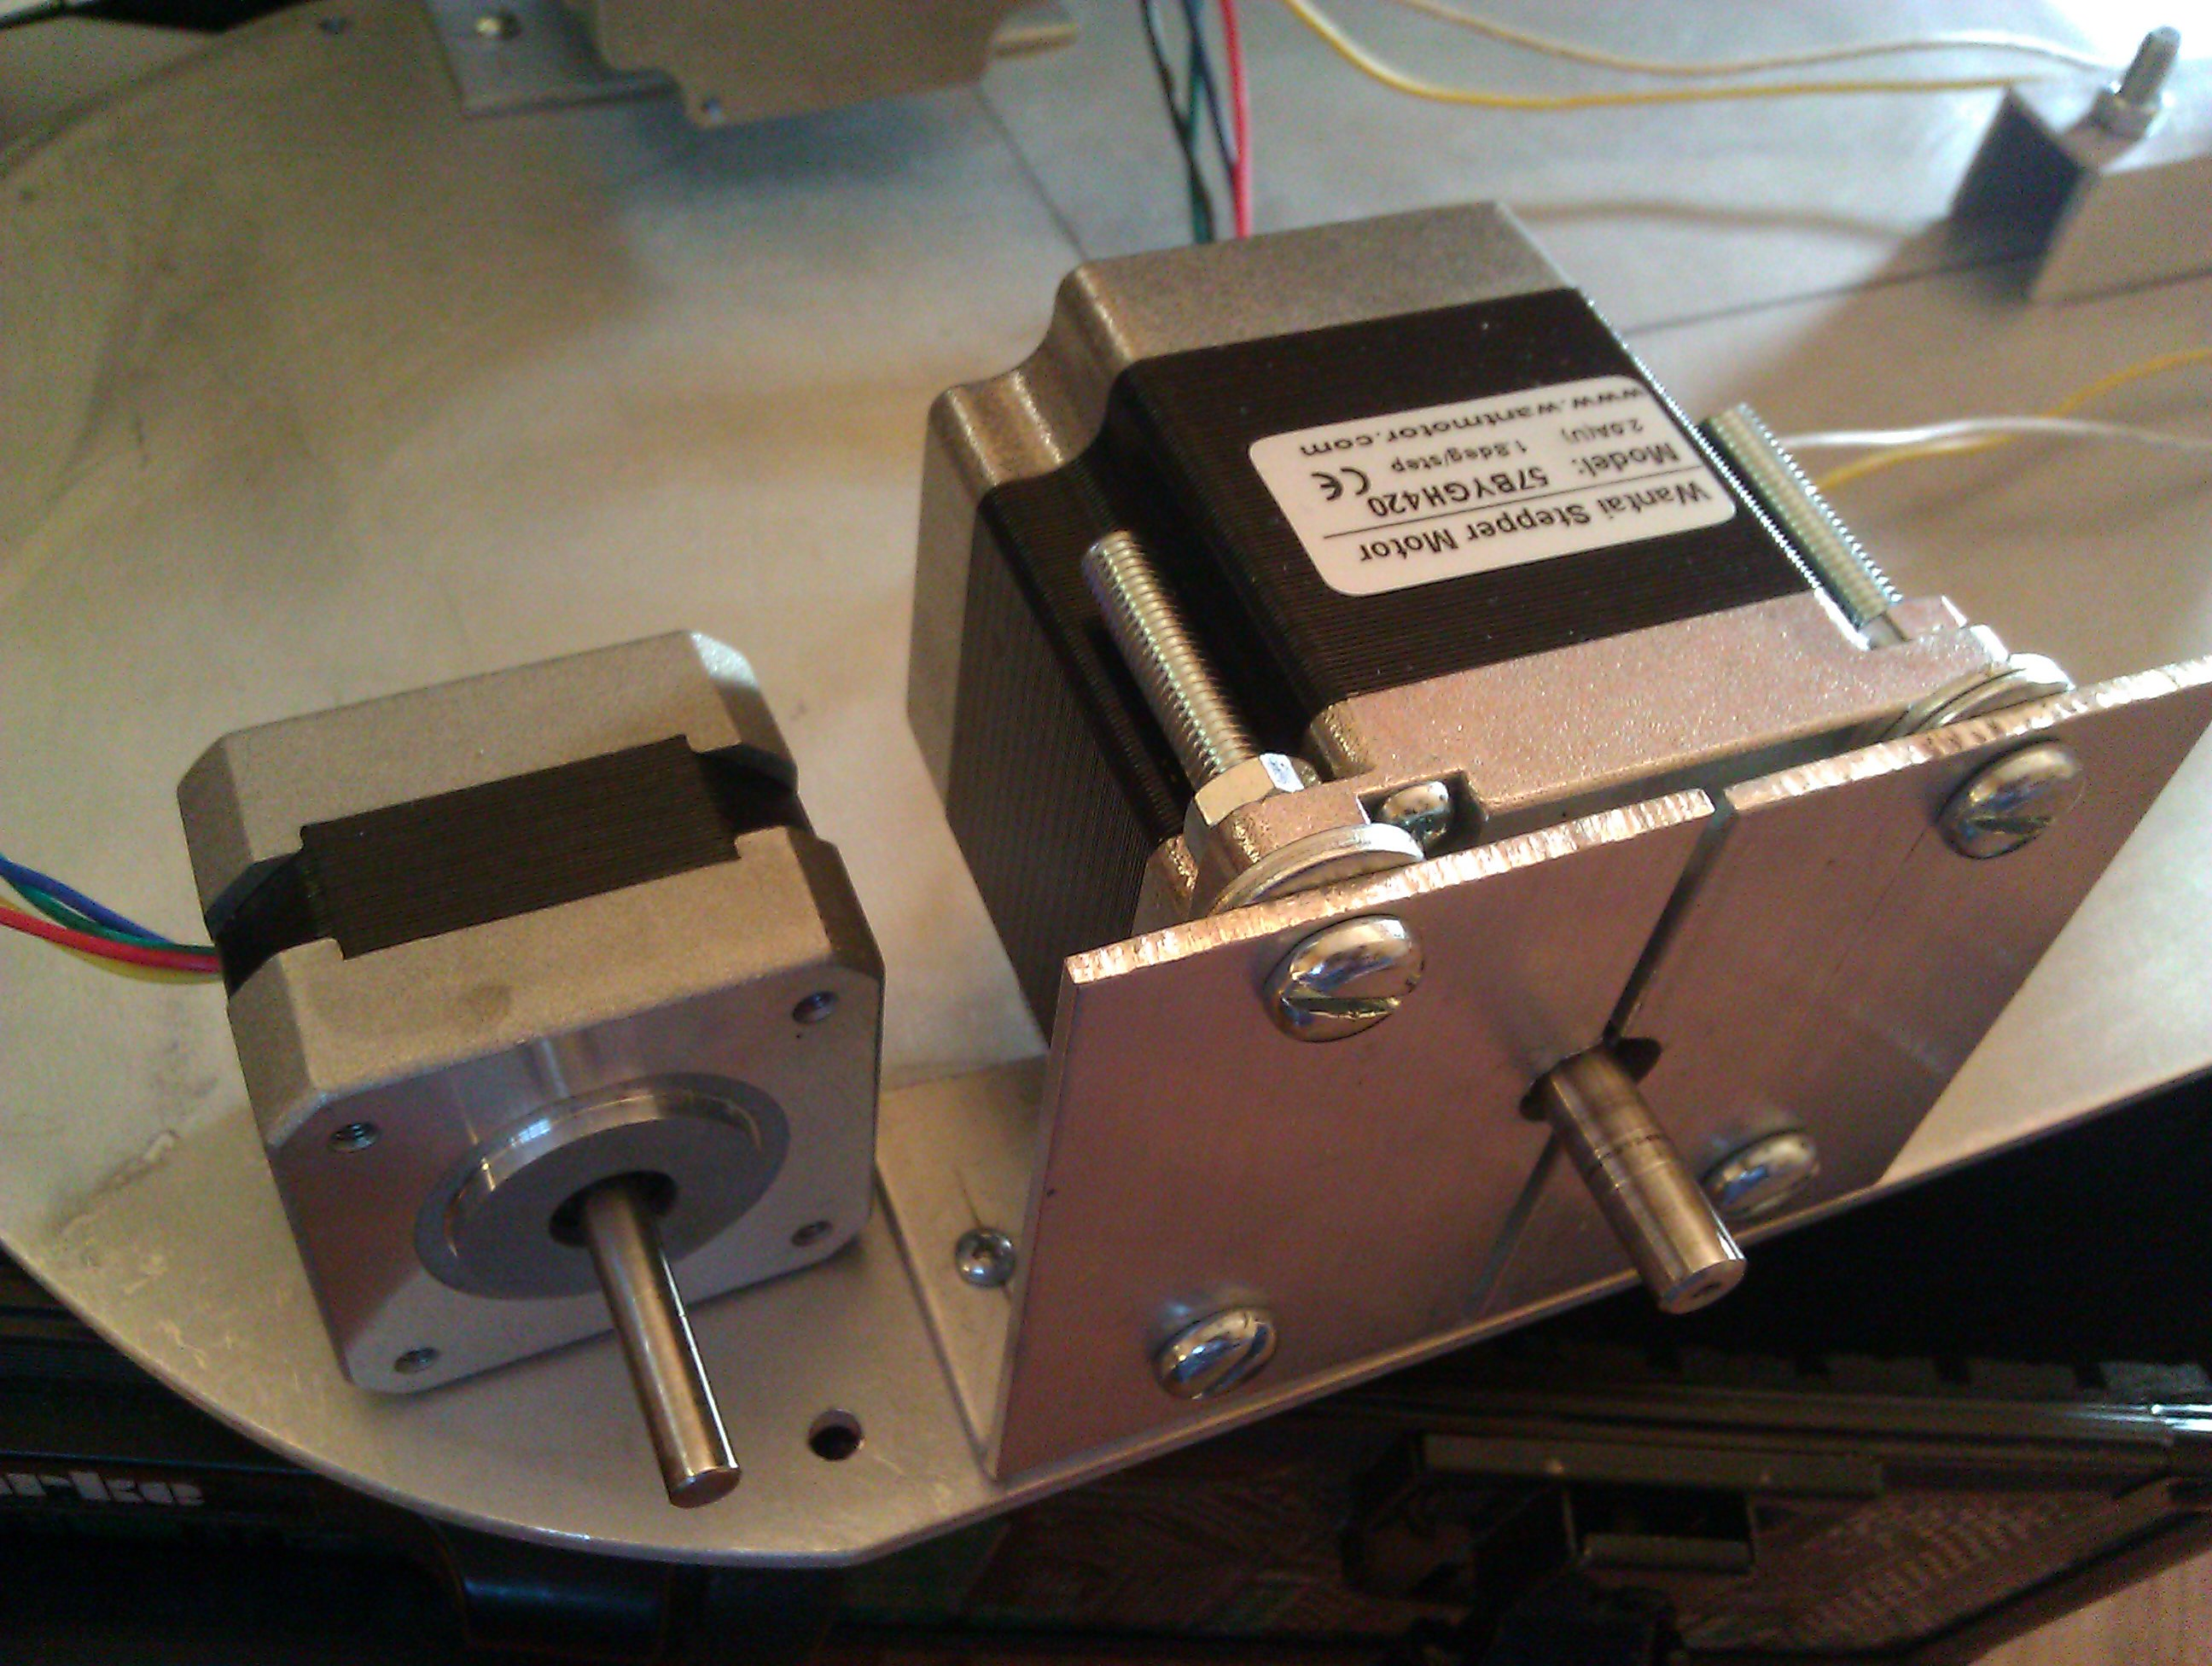
\includegraphics[width=4.0in]  {Images/motor-compare.jpg}
        \caption{New Motor Next to Old Motor}
        \label{New Motor Next to Old Motor}
\end{figure}
These new motors can move the robot much much greater ease than the previous ones, even when trying to turn.  It can now turn in a much smaller space resulting in me being able to reduce the threshold on the sonar sensor setting.
\\Another change made in this iteration was removing the code that used the stepper motor library and instead I wrote my own control code which just sends signal pulses to each stepper motor wire manually.  All this involves is powering each coil in order to turn the motor.  The advantage to performing this manually instead of using the library is that the library does not support braking.  If all of the coils are powered at the same time the magnets actively hold the motor shaft in place, this can help when starting to move as the first part of the motion is already done by holding the shaft in position instead of having to pull it into position at the start of the motion cycle of code.
\subsection{MK-IV Evaluation}
The MK-IV now moves with greater easy and can now turn faster so that it does not drive straight into walls.  It is now configured to avoid objects when it is closer to them.
\\The new issue that has turned up with this iteration of the design is again with the drive system.  This time the h-bridge motor drivers overheat, this is due to the additional load that the new bigger motors draw from the system.  One of them actually burnt out even with a heat sink attached.
\section{MK-V}
The MK-V was focussed on resolving the latest drive system issue.  I tried adding some current limiting resistors which did reduce the temperate by a small amount but the motor drivers still ran too hot.
\\I had then decided to implement a pre-built motor driver into the system, one which is not too expensive.  I found a suitable unit with standard spacing holes in the board which pins can be soldered through in order to fit into the breadboard that is already attached to the robot chassis baseplate for the previous motor driver.  This unit is a Pololu motor driver that operates between 8 and 35 volts which is well within the voltage range of the robot's system.  The new motor driver can also supply 1.2 amps of current to each coil of the motor without the need for cooling, but with proper cooling it can supply up to 2 amps of current which is much more than the h-bridge drivers that had a maximum supply of 1 amp and overheated before that.
\begin{figure}[H]
\centering
        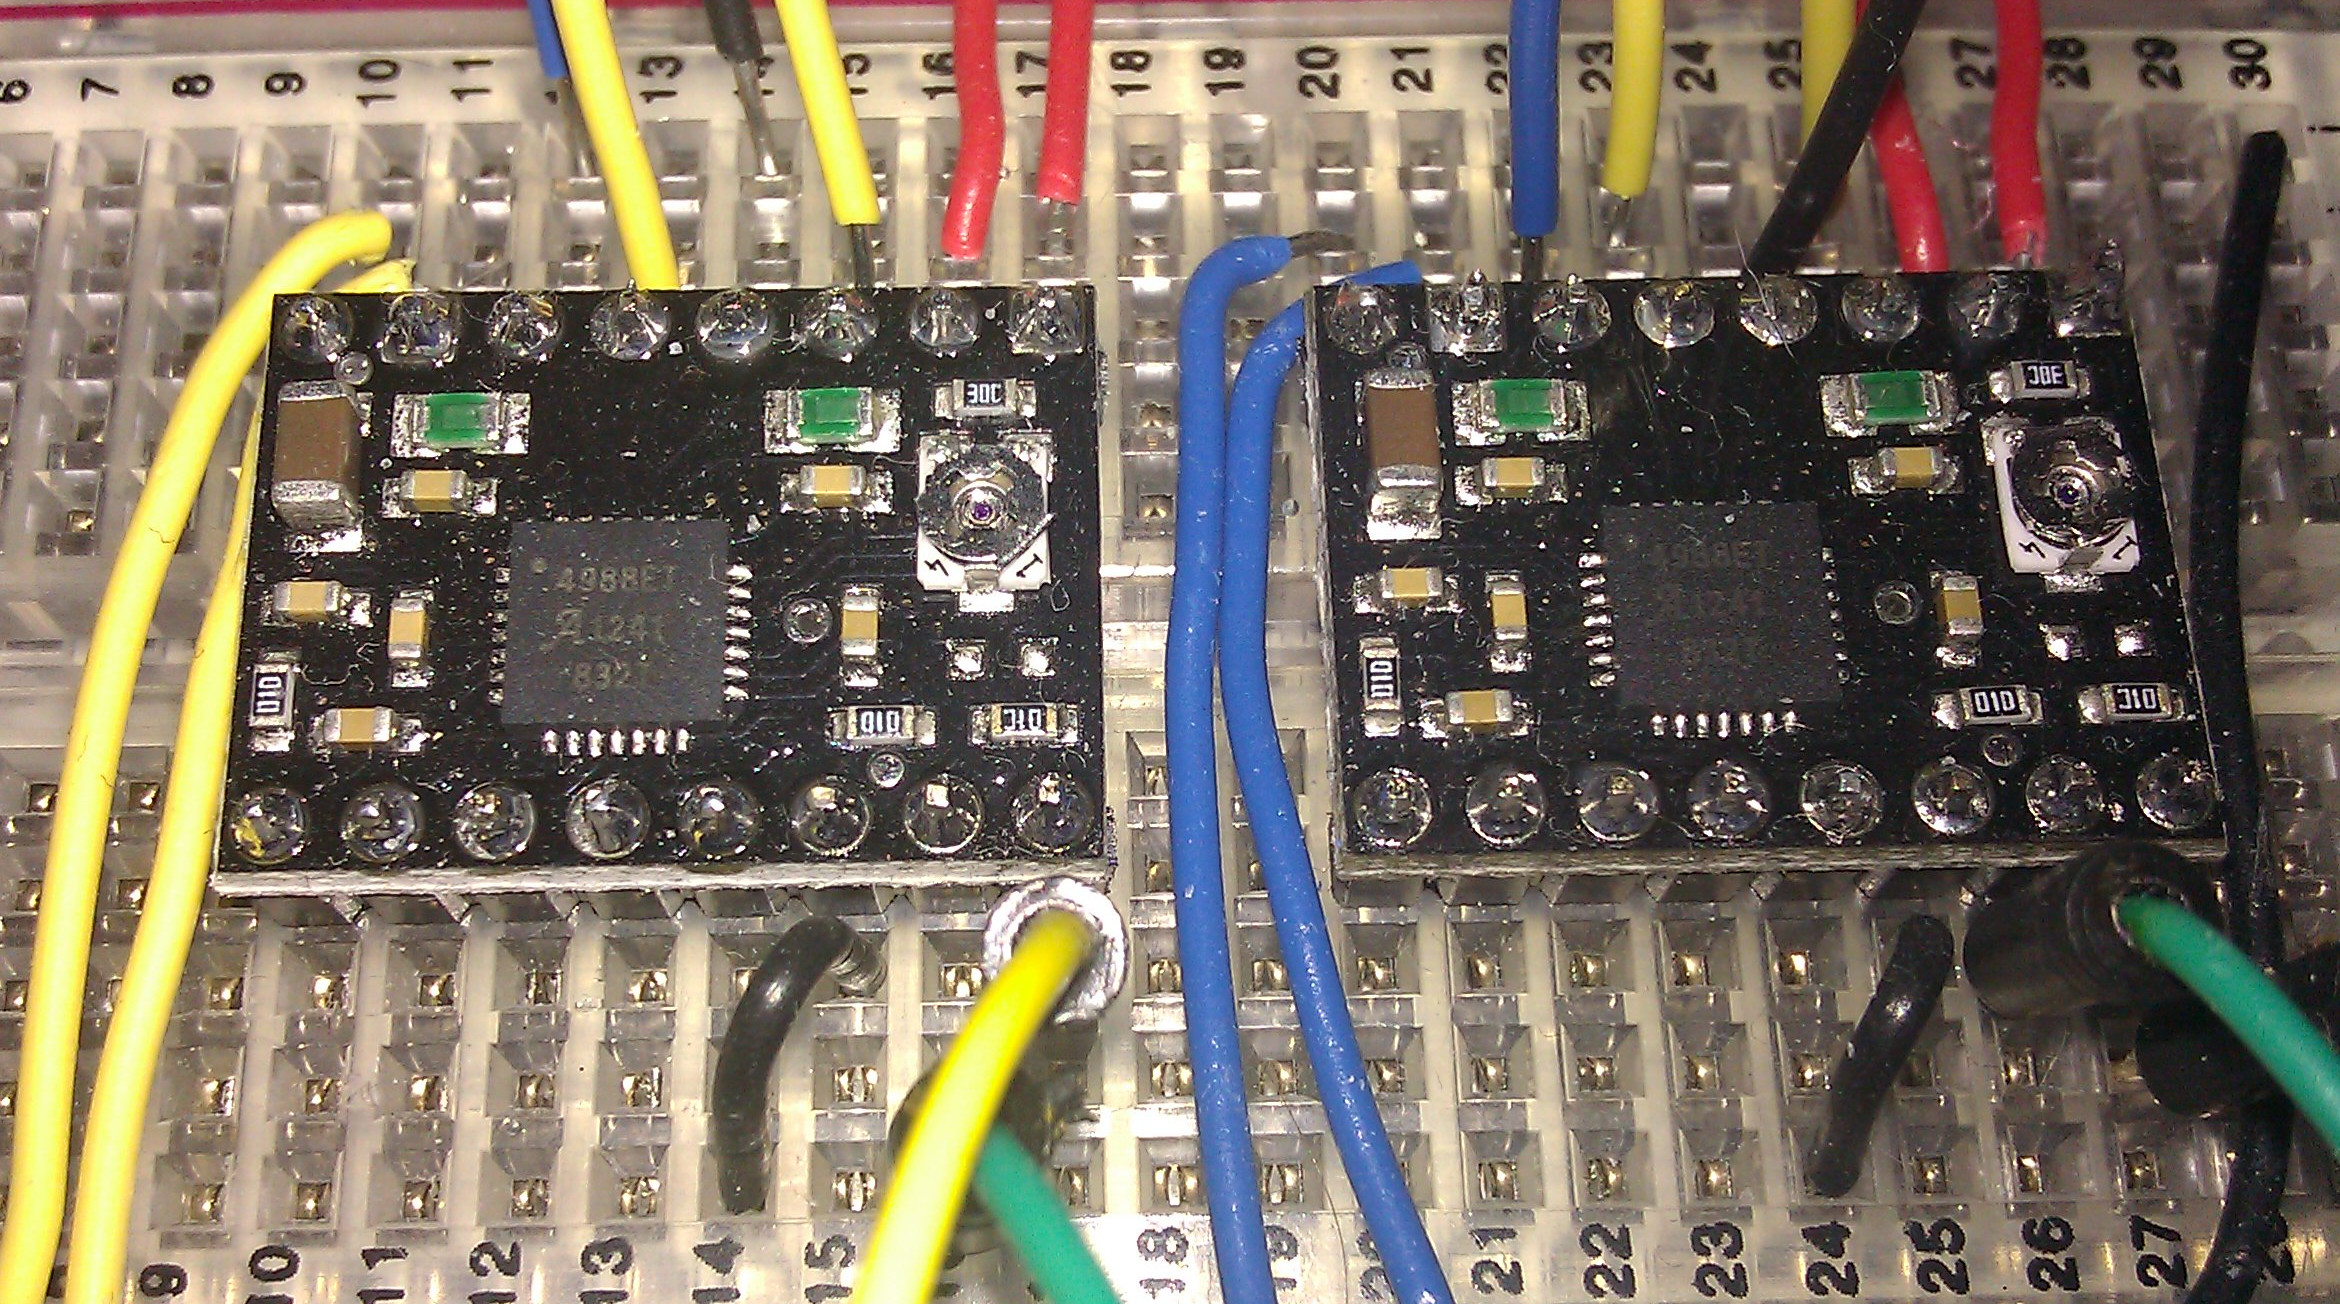
\includegraphics[width=4.0in]  {Images/pololu-motor-driver.jpg}
        \caption{Replacement Motor Driver}
        \label{Replacement Motor Driver}
\end{figure}
With the old driver system I had to manually control the signals to each of the connections of each stepper motor, the new drivers only require a direction signal and a step pulse per motor.  The motor turns a step each time the step pin on the motor driver receives a signal pulse.  This system is less complex to control but has the downside of not being able to brake.  By this I mean that with the previous system I was able to supply current manually to all of the motor connection coils which would hold the motor in it's current position, but with the new drivers it manages the current to the motor coils itself and because of this I cannot specify if I want the motors holding their position rather than just not turning.
\subsection{MK-V Evaluation}
The MK-V robot now drives with greater reliability than previous iterations due to the combination of the bigger stepper motors and the new motor drive boards.
\\The downsides to this iteration is that it can no longer actively brake and it still only uses two sonar sensors to detect obstacles, this means that it still suffers from the cons of using sonar to detect range.

\section{MK-VI}
The MK-VI iteration focused on adding infrared sensors to accompany the sonar sensors.  As previously mentioned in the design section, it was always intended that sonar and infrared would be used together to decrease the number of false readings produced by the sensor system.
The infrared sensors suffer from ambient infrared radiation giving them false readings.  The sonar sensors suffer from echo where the sounds bounces more than once before coming back to the receiver and thus gives a distance reading indicating the object is at a greater distance from the sensor that it actually is in reality.
As the two different types of sensors suffer from different issues the objective is that if one sensor gives a reading that is too far different than the other sensor it is paired with then the robot will discard that reading and request a new set of readings from the sensor pair before making a decision if it should move or not.
\\The sensors were just placed on the front of the robot chassis to begin with, this is for testing purposes.  Sonar sensors are already plugged into small breadboards and the infrared sensors are placed underneath the sonars against the side of the small breadboards.
\begin{figure}[H]
\centering
        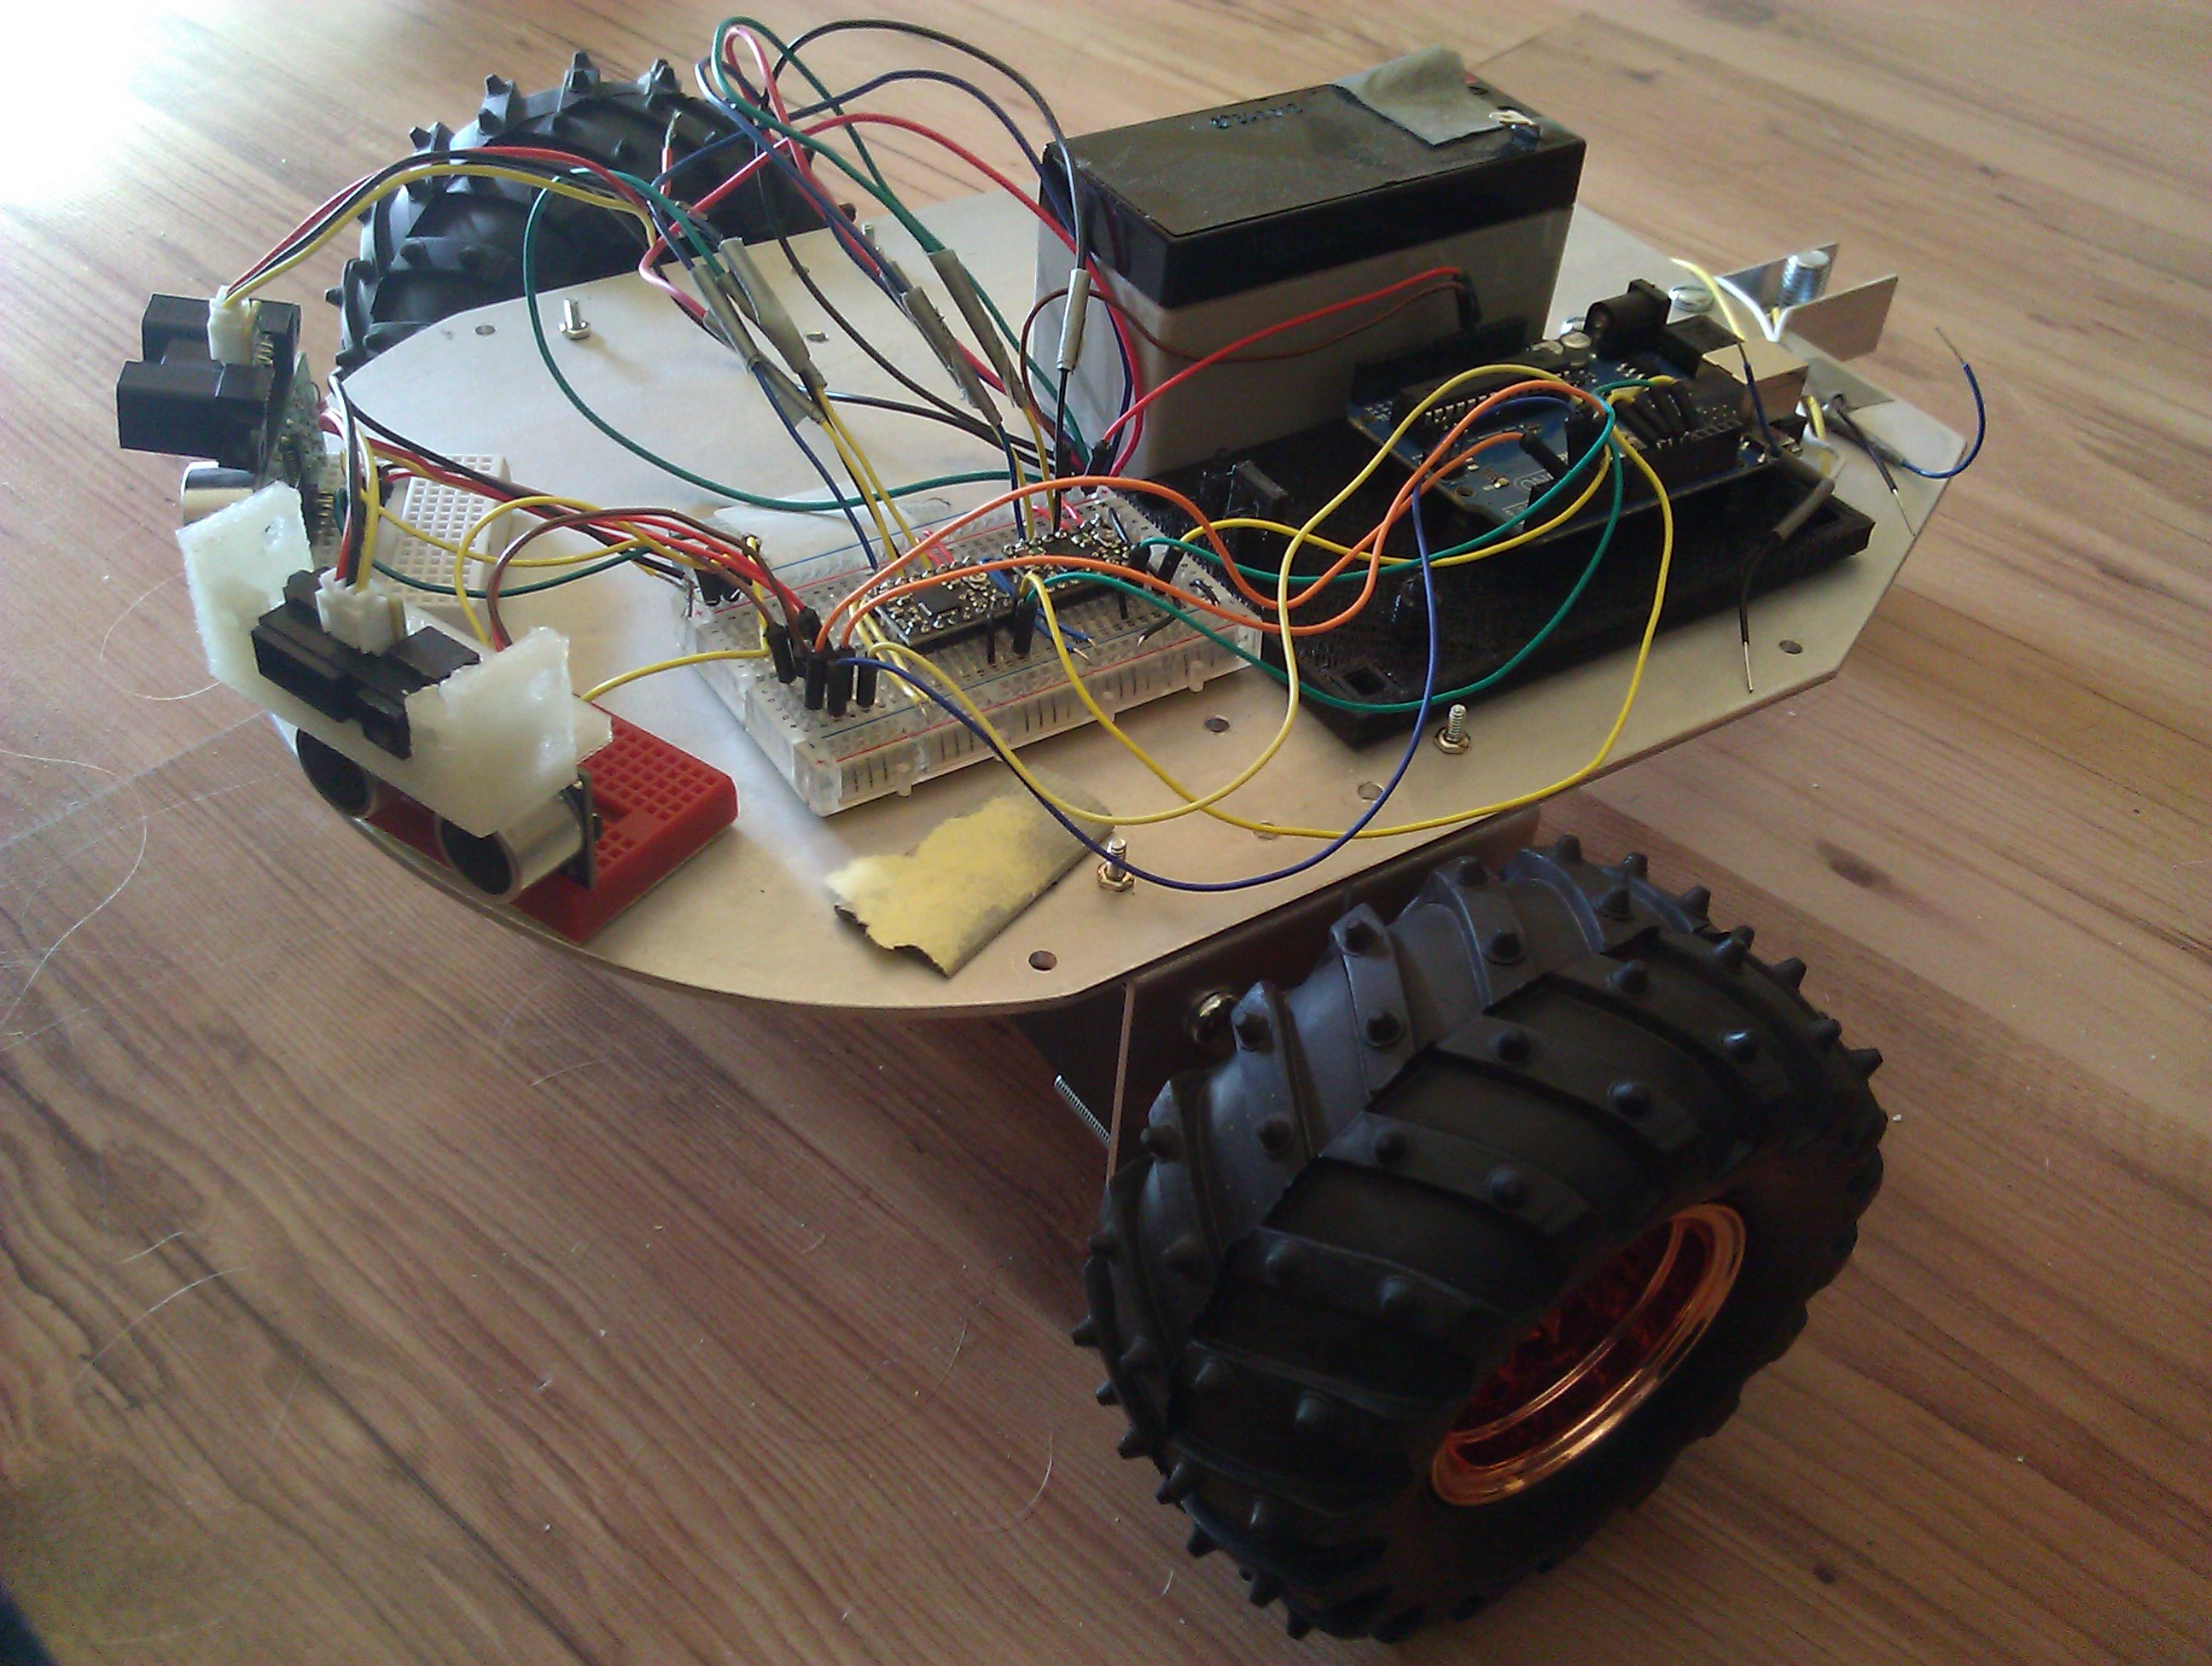
\includegraphics[width=4.0in]  {Images/mk-vi.jpg}
        \caption{MK-VI Robot}
        \label{MK-VI Robot}
\end{figure}
After placing the sensors on the robot I then had to write the code that gathers the sensor data, compares each pair to check if there are any major differences in their readings.  If there are any differences above a threshold value then discard the readings and take a new set.  Once an acceptable set of readings have been taken the robot will use the already existing decision code to determine which direction for the drive system to move the robot in.
To test this new code I put the robot up on blocks so that the wheels did not move the robot, then I put an object at different distances from each sensor in each pair.  This worked very well as the system kept requesting new sensor readings until I moved the objects to roughly the same distance away.
\\The 3D printer was used again to make the sensor mounts which are then attached to the robot chassis and house a sensor in each.
\begin{figure}[H]
\centering
        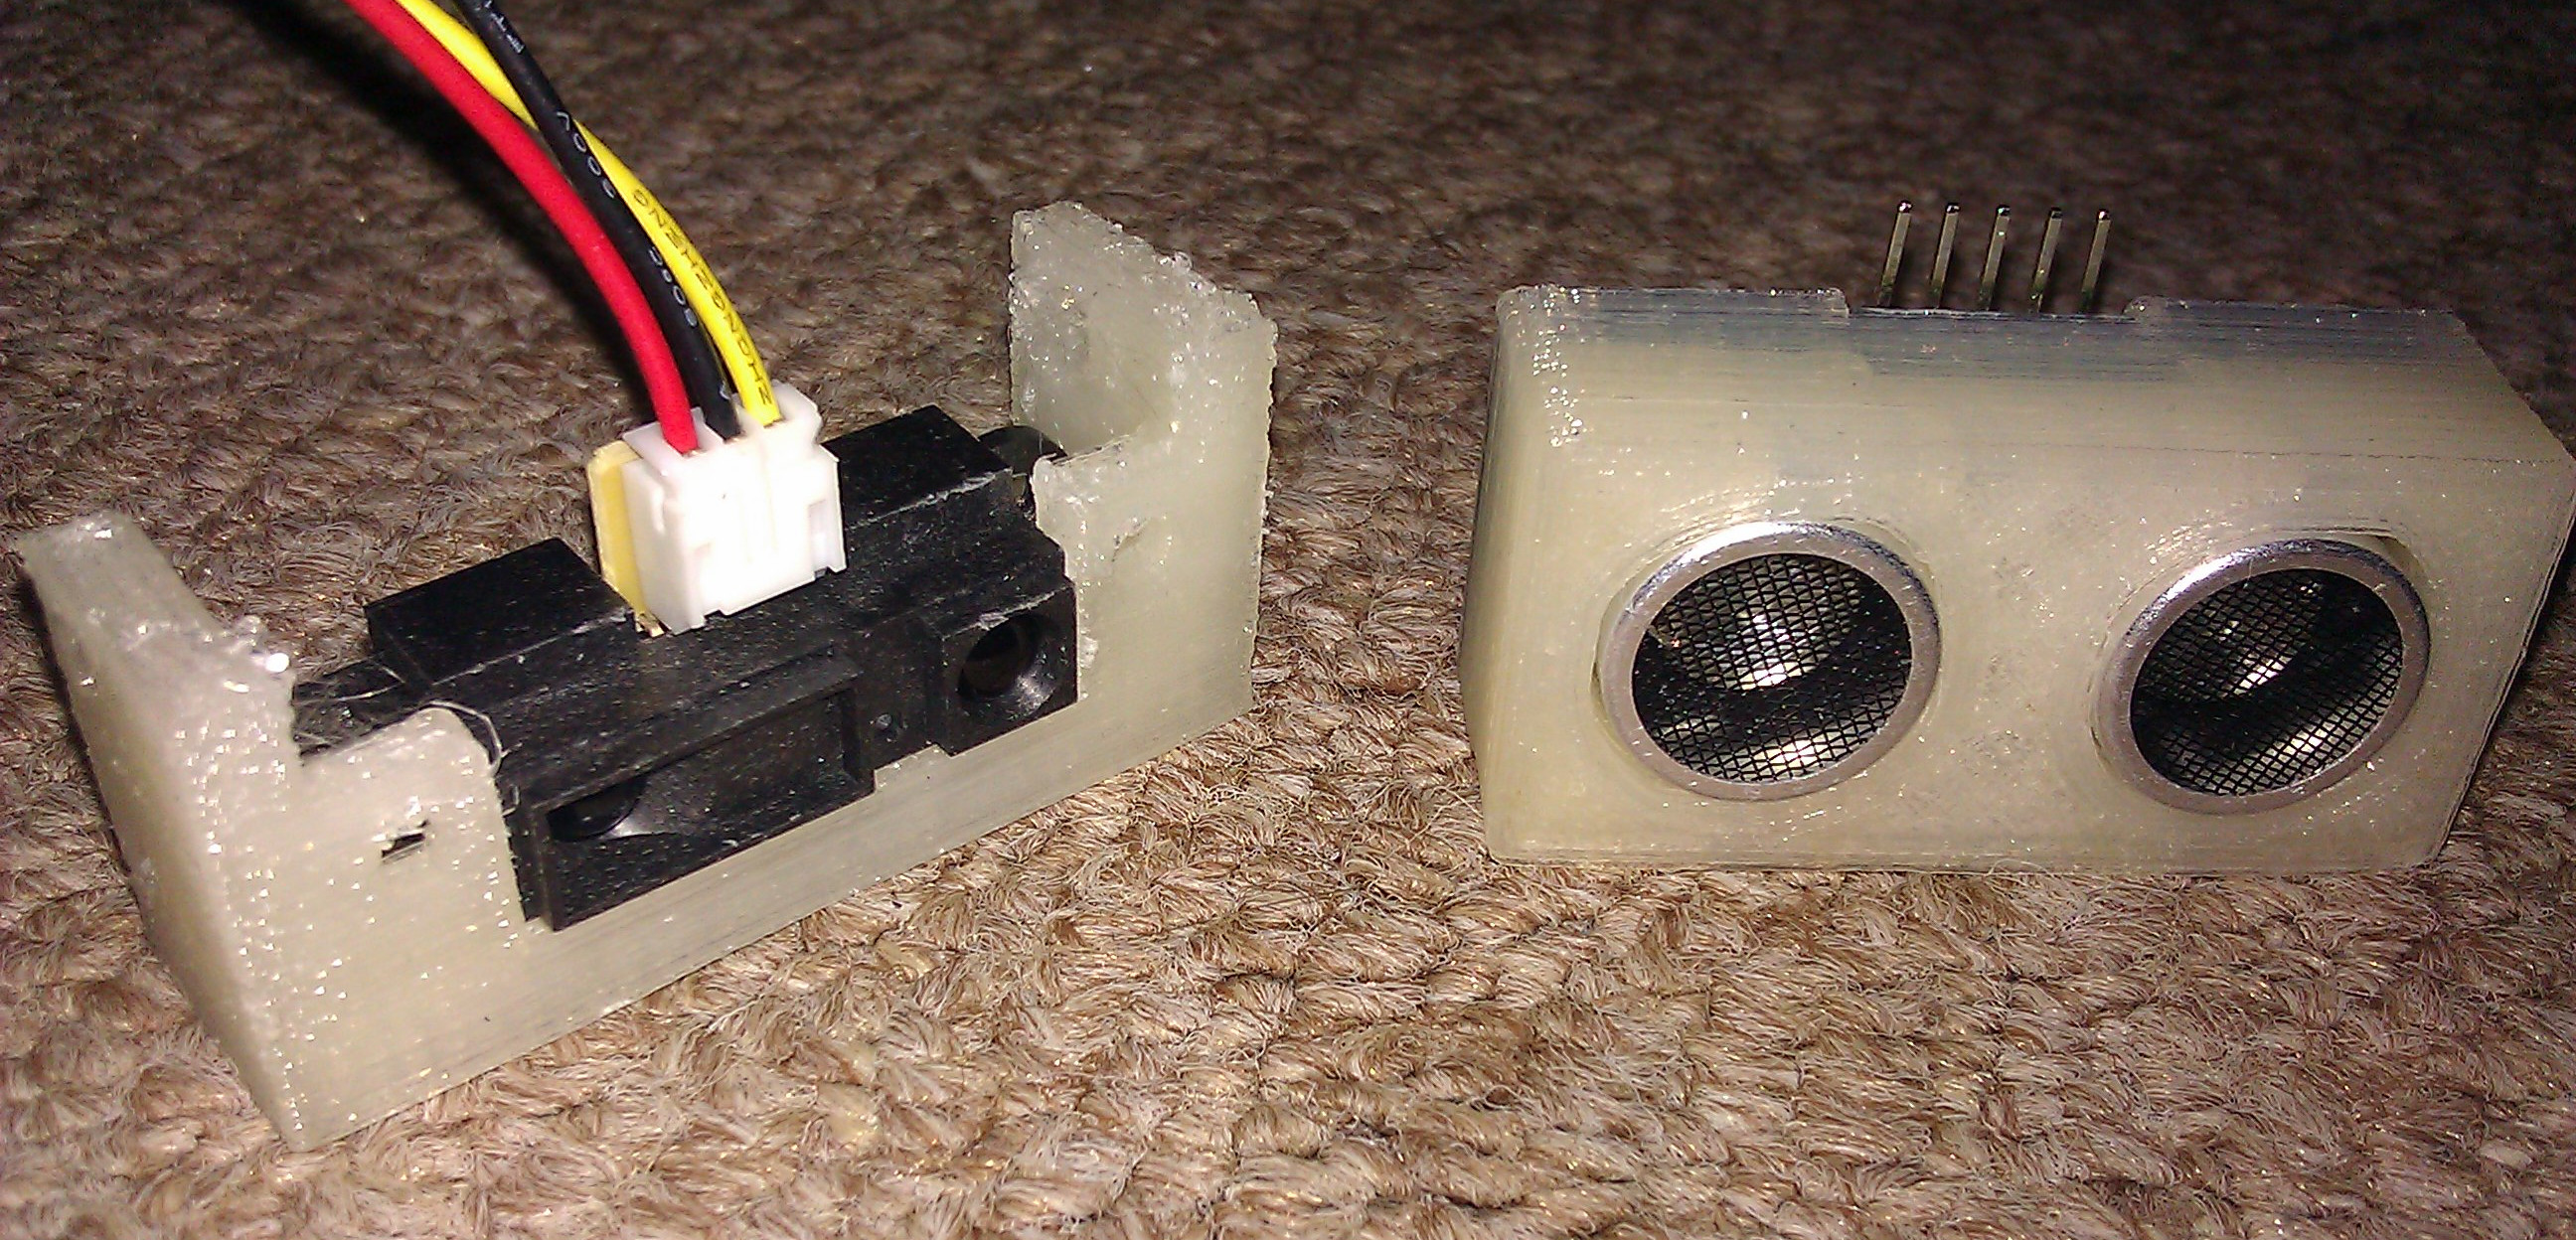
\includegraphics[width=4.0in]  {Images/printed-sensor-mounts.jpg}
        \caption{Printed Sensor Mounts}
        \label{Printed Sensor Mounts}
\end{figure}
